\section{Произведение метрических пространств и арифметика предела.}

\begin{definition}
 Пусть $(E_1,d_1)$, $(E_2,d_2)$ -- два метрических пространства, где $d_1$, $d_2$ -- расстояния в $E_1,$ $E_2$. Для любой пары точек $x = (x_1,x_2)$, $y = (y_1,y_2)$, где $x_1, x_2 \in E_1$, $y_1,y_2 \in E_2$ положим
 \[
  d(x,y):= \max \{ d_1(x_1,y_1), d_2(x_2,y_2)\}.
 \]
\end{definition}

Непосредственно проверяется, что это метрика. Тем самым, мы получаем метрическое пространство $(E, d)$, где $E = E_1 \times E_2$

\begin{mydanger}{\bf !}
    Открытые шары для расстояний $d,d_1,d_2$ будут соответственно обозначаться символами $B,B_1,B_2.$
\end{mydanger}

\begin{lemma}
    Для любой точки $a = (a_1,a_2) \in E$ и любого $r >0$ имеем $ B(a,r )  = B_1(a_1,r_1) \times B_2(a_2, r_2)$.
\end{lemma}
\begin{proof}
    Это сразу следует из определения метрики $d$, $d(x,y):= \max \{ d_1(x_1,y_1), d_2(x_2,y_2)\}.$
\end{proof}

\begin{proposition}\label{continous_of_times}
    Пусть $F,E_1,E_2$ -- метрические пространства, и пусть $f_1:F \to E_1$, $f_2:F \to E_2$ -- отображения. Тогда отображение $f:F \to E_1 \times E_2$, $z \mapsto (f_1(z), f_2(z))$ будет непрерывным в точке $z_0 \in F$, если и только если оба отображения $f_1,f_2$ непрерывны в точке $z_0.$
\end{proposition}
\begin{proof}
    Пусть $p_0 = (f_1(z_0), f_2(z_0))$, покажем, что 
    \[
     f^{-1} (B(p_0, r)) = f_1^{-1}(B(f(z_0) , r)) \cap f_2^{-1}( B(f_2(z_0)), r ).
    \]
Действительно, имеем
\begin{eqnarray*}
  z \in f^{-1} (B(p_0, r)) &\Longleftrightarrow&  f(z) \in B(p_0,r) \\
   &\Longleftrightarrow& (f_1(z), f_2(z)) \in B_1(f(z_0), r) \times B(f_2(z_0), r) \\
   &\Longleftrightarrow& \bigl\{ z \in F\,:\, f_1(z) \in B_1(f_1(z_0), r) \bigr\}  \& \bigl\{ z\in F, :\, f_2(z) \in B_2(f_2(z_0), r) \bigr\} \\
   &\Longleftarrow& z \in f_1^{-1}(B_1(f_1(z_0), r)) \cap f_2^{-1}(B_2(f_2(z_0), r)).
\end{eqnarray*}

Тогда, используя лемму \ref{union_and_cap_of_open}, получаем, что прообраз любого открытого при $f$ открыт, что и доказывает предложение.
\end{proof}

\begin{theorem}
    Пусть $\alpha: \mathbb{R} \times \mathbb{R} \to \mathbb{R}$ -- любая бинарная непрерывная операция на $\mathbb{R}$ относительно метрики $d(x,y) = |x-y|$. Пусть $f,g:E \to \mathbb{R}$ -- отображение из метрического пространства $E$, при этом, для какого-то $A \subseteq E$, $a\in \overline{A}$, $\lim_{x\to a, x \in A}f(x) = a'$, $\lim_{x\to a, x \in A}g(x) = a''$. Тогда $\lim_{x\to a, x \in A}\alpha(f,g) = \alpha(a',a'').$
\end{theorem}

\begin{proof}
    Это сразу следует из определения предела, теоремы \ref{comp_of_continous} и предложения \ref{continous_of_times}.
\end{proof}


\begin{corollary}
    Арифметика предела для функций верна, если функции определены подходящим образом.
\end{corollary}

Напомним, что функция $f:\mathbb{R}^2 \to \mathbb{R}$, где рассматривается обычная метрика на $\mathbb{R}^2$, $\mathbb{R}$, непрерывна в точке $(a,b)$, если для любого $\varepsilon >0$ можно найти такое $\delta >0$, что неравенство 
\[
 \sqrt{(x-a)^2 + (y-b)^2} < \delta
\]
влечёт неравенство $|f(x,y) - f(a,b)|< \varepsilon$. 

(1) Покажем, что $\mathsf{S}:\mathbb{R} \times \mathbb{R} \to \mathbb{R}$, $(x,y) \mapsto x+y$  непрерывно. Если $|x-a|, |y-b| <\delta$, то $ \sqrt{(x-a)^2 + (y-b)^2} < \sqrt{2}\delta < 2 \delta$, и 
\[
 |x+y - (a+b)| = |(x-a) + (y-b)| \le |x-a| + |y-b| < 2 \delta.
\]

Поэтому если $\sqrt{(x-a)^2 + (y-b)^2}<\varepsilon$, то и $|(x+y) - (a+b)|< \varepsilon$, что и означает непрерывность отображения $\mathsf{S}$ в любой точке $(a,b).$

(2) Покажем, что отображение $\mathsf{P}: \mathbb{R} \times \mathbb{R} \to \mathbb{R}$, $(x,y) \mapsto xy$ непрерывно. 

Пусть $|x-a|, |y-b| < \delta$, тогда  $\sqrt{(x-a)^2 + (y-b)^2} < \sqrt{2}\delta < 2 \delta$.

Далее, имеем
\[
 xy -ab =a (y-b) + b(x-a) + (x-a)(y-b),
\]
тогда
\begin{eqnarray*}
   |xy -ab| \le |a| |y-b| + |b||x-a| + |x-a||y-b|  & \le &   |a| \delta + |b| \delta + \delta^2\\
   &=& \delta (|a| + |b| + \delta).
\end{eqnarray*}

Если потребовать, что $\delta <1$, то мы получаем $|xy-ab| < \delta (|a| + |b|+1).$ Таким образом, если задано произвольное $\varepsilon >0$ такое, что $|xy -ab| < \varepsilon$, то возьмём такое $\delta$, что $0 < \delta <1$ и $\delta(1 + |a| + |b|)<\varepsilon$, наконец, пусть $\delta' = 2{\delta}$. Тем самым, мы получаем, что из неравенства $\sqrt{(x-a)^2 + (y-b)^2} < \sqrt{2}\delta < 2 \delta = \delta'$ следует неравенство $|xy - ab| < \varepsilon$, что и показывает непрерывность отображения $\mathsf{P}.$

(3) Покажем, что отображение $h_\lambda: \mathbb{R} \to \mathbb{R}$, $x \mapsto \lambda x$, где $\lambda$ -- фиксированное число, непрерывно. 

Действительно, во-первых, если $\lambda  =0$, то получаем постоянное отображение которое, очевидно, непрерывно. Во-вторых, если $\lambda \ne 0$, то для $\varepsilon >0$ пусть $\delta = \frac{\varepsilon}{|\lambda|}$. Тогда если $|x-a|<\delta < \frac{\varepsilon}{\lambda}$, то $|\lambda||x-a| < \varepsilon$, \ie $|\lambda x - \lambda a| < \varepsilon$, что и доказывает требуемое.

(4) Покажем, что отображение $f:\mathbb{R}/\{0\} \to \mathbb{R}$, $x \mapsto \frac{1}{x}$ непрерывно. То есть нужно показать, что если для заданного $\varepsilon>0$ всегда можно найти такое $\delta>0$, что $|x-a|<\delta$, то $|\frac{1}{x} = \frac{1}{a}|<\varepsilon.$

Пусть $|x-a|<\delta$, тогда, $|a| - |x| \le |a-x| = |x-a| < \delta$, значит $|x|>|a| -\delta$. Далее, для заданного $\varepsilon>0$ мы положим 
\[
0<\delta < \min \left( \frac{|a|}{2}, \varepsilon\frac{|a|^2}{2} \right),
\]
тогда если $|x-a|< \delta$, то $|x|>\frac{|a|}{2}$. Действительно, если $\frac{|a|}{2}< \varepsilon\frac{|a|^2}{2}$, то $|x| > |a| - \delta > \frac{|a|}{2}$. Если же $\frac{|a|}{2}> \varepsilon\frac{|a|^2}{2}$, то $\varepsilon < \frac{1}{|a|}$ и тогда $|x|  > |a| - \delta > |a| -\varepsilon \frac{|a|^2}{2} > |a| -  \frac{1}{|a|}\frac{|a|^2}{2} = |a| - \frac{|a|}{2} = \frac{|a|}{2}.$

Имеем

\[
 \left| \frac{1}{x} - \frac{1}{a} \right| = \frac{|a-x|}{|ax|} \le \frac{2 |a-x|}{|a|^2} < \varepsilon,
\]
что и доказывает непрерывность $f$.





\subsection{Дифференцируемость функций от одной переменной.}

Пусть $n=m=1$, тогда любое линейное отображение $\mathscr{L}:\mathbb{R} \to \mathbb{R}$ имеет простой вид $\mathscr{L}(x) = kx$, $k \in \mathbb{R}$ -- фиксированное число, и $||\m{h}|| : = |h|$ -- обыкновенный модуль. Тогда, согласно определению, функция $f:\mathbb{R} \to \mathbb{R}$ дифференцируема в точке $x_0$, если существует такое \textbf{число} $k\in \mathbb{R}$, что
\[
 f(x_0+h) = f(x_0)+kh + o(h), \qquad h \to 0.
\]

\begin{mydanger}{\bf{!}}
 Это число $k$, вообще говоря, зависит от выбранной точки $x_0$! 
\end{mydanger}~

Рассмотрим примеры.

\begin{example}
    Пусть $f(x) = x^2$, покажем, что она дифференцируема всюду. Действительно, имеем
     \begin{eqnarray*}
         f(x+h) &=& (x+h)^2 \\
         &=& x^2 + 2xh + h^2 \\
        &=& f(x) + 2x \cdot h + o(|h|).
     \end{eqnarray*}

Таким образом, дифференциал определяется следующим образом: $\mathrm{d}f_{x_0} = 2x_0$ для любого $x_0 \in \mathbb{R}$.

Это же равенство можно записать ещё так:
\[
 (x+h)^2 \approx x^2 + 2xh,
\]
при этом, чем меньше будет $h$, тем точнее будет результат. Например, $1.1^2 =1.21$, а по нашей формуле $1.1^2 = (1+0.1)^2 \approx 1^2+ 2\cdot 1 \cdot 0.1 = 1.2.$
\end{example}

\begin{example}
Мы рассмотрим функцию уже от двух переменных $F: \mathbb{R}^2 \to \mathbb{R}$, $F(x_1,x_2): = (x_1 + x_2)^2$, где $\m{x} = (x_1, x_2)$. Покажем, что она тоже всюду дифференцируема. Пусть $\m{h}= (h_1,h_2)$, тогда получаем
\begin{eqnarray*}
    F(\m{x} + \m{h}) &=& F((x_1 +h_1) + (x_2 + h_2) ) \\
    &=& ((x_1 +h_1) + (x_2 + h_2) )^2 \\
    &=& ((x_1 + x_2) + (h_1 + h_2))^2 \\
    &=& (x_1 + x_2)^2 + 2(x_1 + x_2)(h_1 + h_2) + (h_1 + h_2)^2 \\
    &=& F(\mathbf{x}) + \begin{pmatrix}
        2(x_1 + x_2) & 2(x_1 + x_2)
    \end{pmatrix} \begin{pmatrix}
        h_1 \\ h_2
    \end{pmatrix} + o(||\m{h}||).
\end{eqnarray*}

Прокомментируем, что тут написано. Во-первых, если $\m{h} \to 0$, то, по Лемме \ref{||h||->0}, $h_1, h_2 \to 0$. Мы должны показать, что $(h_1+h_2)^2 \in o(||\m{h}||)$, \ie $\lim_{h_1 \to 0, h_2 \to 0} \frac{(h_1 + h_2)^2}{\sqrt{h_1^2 + h_2^2}} = 0$. Применим полярную систему координат $h_1 = \rho \cos \varphi$, $h_2 = \rho \sin \varphi$, тогда $\rho = \sqrt{h_1^2 + h_2^2} \to 0$.

Имеем
\begin{eqnarray*}
    \lim_{h_1 \to, h_2 \to 0} \frac{(h_1 + h_2)^2}{\sqrt{h_1^2 + h_2^2}} &=& \lim_{\rho \to 0} \frac{\rho ^2 + 2\rho^2 \cos \varphi \sin \varphi }{\rho} \\
    &=& \lim_{\rho \to 0} \rho \cdot \left(1 + \sin 2\varphi \right) \\
    &=& 0,
\end{eqnarray*}
поэтому $(h_1 + h_2)^2 \in o(||\m{h}||).$

Во-вторых, произведение $2(x_1 + x_2)(h_1 + h_2)$ можно записать в виде произведения матриц
\[
 \begin{pmatrix}
        2(x_1 + x_2) &2(x_1 + x_2)
    \end{pmatrix} \begin{pmatrix}
        h_1 \\ h_2
    \end{pmatrix} = 2(x_1 + x_2)(h_1+h_2),
\]
таким образом, наше отображение $F$ -- дифференцируемо, его дифференциал в точке $(a, b)$ задаётся матрицей размера $1\times 2$:
\[
 \mathrm{d}F_{(a,b)} = \begin{pmatrix}
     2(a+b) & 2(a+b)
 \end{pmatrix}.
\]

\end{example}

Вернёмся к функциям от одной переменной.

Запись $f(x_0+h) = f(x_0)+kx_0 + o(h),$ $h \to 0$ означает также, что
\[
 k = \lim_{h \to 0} \frac{f(x_0 +h) - f(x_0)}{h}
\]
таким образом, дифференцируемость функции равносильна существованию этого предела.

\begin{definition}
    \textit{Производная} функции $f(x)$ в точке $x_0$ -- это предел 
    \[
 \lim_{h\to 0} \frac{f(x_0 + h) - f(x_0)}{h},
    \]
    который принято обозначать одним из следующих образом: $f'(x_0)$, $\frac{d f}{dx}(x_0)$, а если -- $x$ это параметр времени, который обозначается обычно через $t$, то производную также обозначают как $\dot{f}(t_0)$.
\end{definition}

\begin{mydanger}{\bf{!}}
    Дифференциал -- это линейная часть приращения функции, а производная -- это предел отношения приращения функции к приращению аргумента при приращении аргумента, стремящемся к нулю. \textbf{Поэтому это не одно и тоже!!!}
\end{mydanger}


\begin{theorem}\label{diff=contionous(for one varibale)}
    Если функция $f(x)$ дифференцируема в точке $x_0$, то она непрерывна в этой точке.
\end{theorem}

Нам нужно показать, что $\lim_{x \to x_0}f(x) = f(x_0)$, так как значение $f(x_0)$ по определению определено. Пусть $x:=x_0 +h$, тогда если $h \to 0$, то $x \to x_0$ и тогда из определения производной в точке $x_0$ следует, что существует предел
\[
 f'(x_0) = \lim_{x\to x_0} \frac{f(x) - f(x_0)}{x-x_0}.
\]

Имеем
\[
 f(x) - f(x_0) = \frac{f(x) - f(x_0)}{x-x_0}(x-x_0),
\]
тогда
\begin{eqnarray*}
     \lim_{x \to x_0} (f(x) - f(x_0))  &=& \lim_{x \to x_0}\frac{f(x) - f(x_0)}{x-x_0}(x-x_0) \\
     &=& f'(x_0) \lim_{x \to x_0}(x-x_0) \\
     &=& 0,
\end{eqnarray*}
\ie $\lim_{x \to x_0} f(x) = f(x_0)$, что и означает её непрерывность.\\

\begin{mydanger}{\bf{!}}
    В обратную сторону это неверно! То есть если функция непрерывна, то это вовсе не означает, что она дифференцируема.
\end{mydanger}





\chapter{Анализ в $\mathbb{R}^n$}

\section{Сходимость в $\mathbb{R}^n$}



Для доказательства обобщённой теоремы Больцано--Вейерштрасса и вообще в дальнейшем нам понадобится следующее неравенство

\begin{lemma}\label{m<d<M}
Для любых $x_1,\ldots, x_n \in \mathbb{R}$ 
\[
\max_{1 \le k \le n} |x_k| \le \sqrt{\sum_{k=1}^n x_k^2} \le \sqrt{n} \max_{1\le k \le n} |x_k|.
\]
\end{lemma}
\begin{proof}
 
Действительно, перенумеруем все $x_i$ так, чтобы $x_1^2 \le x_2^2 \le \ldots \le x_n^2$, \ie $\max_{1 \le k \le n} |x_k| = x_n$. Но тогда получаем
\[
 \sqrt{x_1^1 + \cdots + x_n^2} \le n x_n^2, 
\]
и 
\[
 x_n^2 \le \sqrt{x_1^1 + \cdots + x_n^2},
\]
что и даёт требуемое неравенство.    
\end{proof}

Для любого вектора $\m{v} = (v_1,\ldots, v_n)^\top \in \mathbb{R}^n$, мы положим 
\[
 \| \m{v} \| : = \sqrt{ v_1^ + \cdots + v^n},
\]
это число называют \textit{нормой} или \textit{длиной} вектора $\m{v}.$




Зафиксируем обозначения. Для каждого элемента $\m{x}_m$ последовательности $\{\m{x}\}$, положим $\m{x}_m = (x_{1m}, x_{2m}, \ldots, x_{nm})^\top$ для каждого $m \ge 1$. Таким образом, всю последовательность можно представить в виде бесконечной матрицы
   \[
    \m{x} = (\m{x}_1,\ldots, \m{x}_m, \ldots,) = \begin{pmatrix}
        x_{11} & x_{12} & \ldots & x_{1m} & \ldots \\
        x_{21} & x_{22} & \ldots & x_{2m} & \ldots \\
        \vdots & \vdots & \ddots & \vdots & \ddots \\
        x_{n1} & x_{n2} & \ldots & x_{nm} & \ldots
    \end{pmatrix}
   \]

\begin{lemma}
    Если $(\m{x}_m)$ последовательность в $\mathbb{R}^n$ такая, что $\lim_{m \to \infty}\m{x}_m = \m{a}$, то она сходится по координатно, \ie $\lim_{m\to \infty}x_{km} = a_k$, где $\m{a} = (a_1, \ldots, a_n)^\top.$
\end{lemma}

\begin{proof}
Согласно неравенству (\ref{m<d<M}) для каждого $1 \le k \le n$, $|x_{km} - a_k| \le d(\m{x}_m, \m{a})<r$.

Имеем 
    \begin{eqnarray*}
        \lim_{m \to \infty} \m{x}_m = \m{a} &\Longleftrightarrow& \forall \varepsilon >0 \, \exists M : \forall m >M, \, d(\m{x}_m, \m{a}) = ||\m{x}_m - \m{a}|| < \varepsilon \\
        &\Longleftrightarrow& \forall\, 1 \le k \le n,\, |x_{km} - a_k| < \varepsilon \\
        &\Longleftrightarrow & \lim_{m \to \infty}x_{km} = a_k,\, 1 \le k \le n,
    \end{eqnarray*}
    что доказывает требуемое.
\end{proof}


\begin{theorem}[\textbf{Обобщённая теорема Больцано--Вейерштрасса}]\label{genB-W}
    Рассмотрим $\mathbb{R}^n$ с обычной метрикой $d$, и пусть имеется такая последовательность $\{\m{x}_m\}$, элементы которой целиком лежат в каком-то шаре $B(\m{a},r)\subseteq \mathbb{R}^n$, тогда в ней имеется сходящаяся подпоследовательность.
\end{theorem}
\begin{proof}

    Пусть $\{\m{x}_m\} \subseteq B(\m{a},r)$, тогда $d(\m{x}_m, \m{a})<r$, но тогда согласно (\ref{m<d<M}),
    \[
     |x_{km} - a_k| \le \max_{1\le k \le n}| x_{km} - a_{k}  | \le d(\m{x}_m, \m{a})<r,
    \]

Так как $\m{a} =(a_1,\ldots, a_n)^\top$ --- фиксированная точка, то числовая последовательность $\{x_{km}\}$ ограничена при каждом $m$ и каждом $1\le k \le n$. Тогда по теореме Больцано--Вейерштрасса (Теорема \ref{B-W}) в последовательности $(x_{1m})$ можно найти сходящуюся подпоследовательность $(x_{1m_{t1}}) \subseteq (x_{1m})$, где $t_1$ пробегает какое-то множество индексов $T_1$. Рассмотрим теперь подпоследовательность $(x_{2m_{t_1}})$ последовательности $(x_{2m})$, которая также ограничена, значит, в ней можно найти сходящуюся подпоследовательность $(x_{2m_{t_2}})$, где $t_2$ пробегает какое-то множество индексов $T_2 \subseteq T_1$. Продолжая таким образом, мы в итоге получим набор подпоследовательностей
\[
 \{(x_{1m_{t_1}}), (x_{2m_{t_2}}), \ldots, (x_{nm_{t_n}})\},
\]
где каждый $t_k$ пробегает множество индексов $T_k$, при этом $T_n \subseteq T_{n-1} \subseteq \cdots \subseteq T_2 \subseteq T_1.$

Тогда положим 
\[
  \m{x}' = \begin{pmatrix}
      (x_{1m_{t_n}}) \\
      (x_{2m_{t_n}}) \\
      \vdots \\
      (x_{nm_{t_n}})
  \end{pmatrix},
\]
что и будет сходящейся подпоследовательностью.    
\end{proof}










\section{Дифференцируемость}

Напомним, что векторное пространство $\mathbb{R}^n$ это просто набор $\{(x_1,\ldots, x_n)^\top\}$ столбцов, которые можно покомпонентно складывать и умножать на число. Выделяется особый набор таких столбцов $\mathbb{e} = \{\mathbf{e}_1, \ldots, \mathbf{e}_n\}$, где $\mathbf{e}_1 = (1,0, \ldots, 0)^\top, \ldots, \mathbf{e}_n = (0,0,\ldots, 1)^\top$. Множество таких столбцов называется \textit{стандартным базисом} для $\mathbb{R}^n$. Имеют место очевидные равенства, возьмём $\mathbf{x} = (x_1,\ldots, x_n)^\top \in \mathbb{R}^n$, тогда ясно, что 
\[
\begin{pmatrix}
    x_1 \\ \vdots \\x_n 
\end{pmatrix} = x_1 \begin{pmatrix}
    1 \\ \vdots \\ 0
\end{pmatrix} + \cdots + x_n \begin{pmatrix}
    0 \\ \vdots \\1
\end{pmatrix}
\]

\textit{Линейное отображение} $\mathscr{L}:\mathbb{R}^n \to \mathbb{R}^m$ -- это такое отображение, что $\mathscr{L}(\alpha \m{x} +\beta \m{y} ) = \alpha \mathscr{L}(\m{x}) +\beta \mathscr{L}(\m{y})$, где $\m{x,y} \in \mathbb{R}^n$, $\alpha, \beta \in \mathbb{R}.$ 

Любое линейное отображение $\mathscr{L}:\mathbb{R}^n \to \mathbb{R}^m$ удобно задавать матрицей $L$. Так как оно линейно, то достаточно знать образы базисных векторов. Действительно, пусть
\[
 \mathscr{L}: \begin{pmatrix}
     1 \\ 0 \\ \vdots \\ 0
 \end{pmatrix} \mapsto \begin{pmatrix}
     a_{11} \\ a_{21} \\ \vdots\\ a_{m1}
 \end{pmatrix}, \qquad
  \mathscr{L}: \begin{pmatrix}
     0 \\ 1 \\ \vdots \\ 0
 \end{pmatrix} \mapsto \begin{pmatrix}
     a_{12} \\ a_{22} \\ \vdots\\ a_{m2}
 \end{pmatrix}, \quad \ldots, \quad \mathscr{L}: \begin{pmatrix}
     0 \\ 0 \\ \vdots \\ 1
 \end{pmatrix} \mapsto \begin{pmatrix}
     a_{1n} \\ a_{2n} \\ \vdots\\ a_{mn}
 \end{pmatrix}
\]
тогда матрица принимает вид
\[
 L = \begin{pmatrix}
     a_{11} & a_{12} & \ldots & a_{1n} \\
     a_{21} & a_{22} & \ldots & a_{2n} \\
     \vdots & \vdots & \ddots & \vdots \\
     a_{m1} & a_{m2} & \ldots& a_{mn}
 \end{pmatrix}
\]

\begin{figure}[h!]
    \centering
    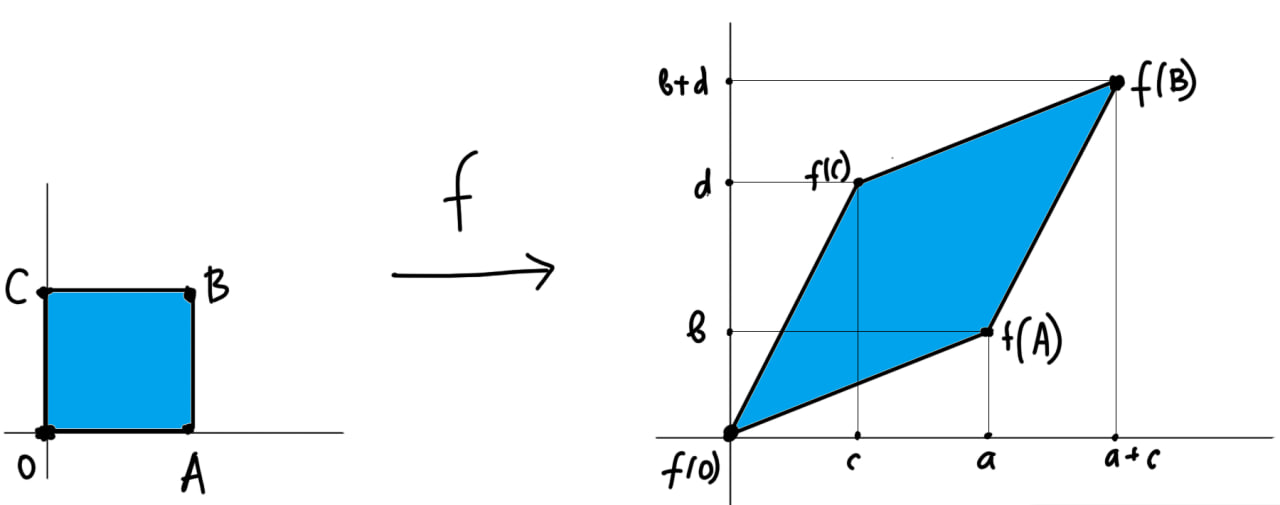
\includegraphics[scale = 0.5]{images/linear_map.jpg}
    \caption{Линейное отображение $f:\mathbb{R}^2 \to \mathbb{R}^2$, которое задаётся матрицей $A = \begin{pmatrix}
        a & c \\
        b & d
    \end{pmatrix}.$}
    \label{linear_map}
\end{figure}

Разумеется, не все отображения линейны. Однако некоторые из них \textit{локально} очень похожи на линейные. Чтобы формализовать эту идею, вводят понятие дифференцируемости.


\begin{definition}\label{diff_of_map(function)}
    Пусть $\mathbb{R}^n$, $\mathbb{R}^m$ -- векторные пространства с евклидовой нормой $\|\cdot \|$, $\mathscr{U} \subseteq \mathbb{R}^n$ -- открытое подмножество. Говорят, что отображение $F: \mathscr{U} \to \mathbb{R}^m$ \textit{дифференцируемо} в точке $\m{v} \in \mathbb{R}^n$, если существует зависящее от точки $\m{v}$ такое линейное отображение $\mathrm{d}F_{\mathbb{v}}:\mathbb{R}^n \to \mathbb{R}^m$, что
    \[
     F(\m{v} + \m{h})  = F(\m{v}) + \mathrm{d}F_\m{v}(\m{h}) + o(\|\m{h}\|),
    \]
где $o(\|\m{h}\|)$ -- вектор, норма которого при $\m{h} \to \m{0}$ бесконечно мала по сравнению с нормой $\|\m{h}\|$.

Другими словами, 
\[
     F(\m{v} + \m{h})  = F(\m{v}) + \mathrm{d}F_\m{v}(\m{h}) + \omega(\m{h}),
    \]
    где 
    \[
     \lim_{\m{h} \to \m{0}} \frac{\| \omega(\m{h})\|}{\| \m{h} \|} = 0.
    \]
Если отображение дифференцируемо в каждой точке $\mathscr{U}$, то говорят, что оно дифференцируемо на $\mathscr{U}$.

Линейное отображение $\mathrm{d}F_\m{v}$ называется \textit{дифференциалом отображения} в точке $\mathbb{v}$. 
\end{definition}

Прежде всего, мы должны убедиться, что линейные отображения тоже дифференцируемы.

\begin{lemma}
    Любое линейное отображение $\mathscr{L}: \mathbb{R}^n \to \mathbb{R}^m$ дифференцируемо
\end{lemma}
\begin{proof}
    Действительно, так как $\mathscr{L}$ -- линейное, то для любых $\m{x,h} \in \mathbb{R}^n$,
    \[
     \mathscr{L}(\m{x}+\m{h}) = \mathscr{L}(\m{x}) + \mathscr{L}(\m{h}),
    \]
    полагая теперь, что $\mathrm{d}\mathscr{L}_\mathbf{x}:=\mathscr{L}$, и так как нулевая функция $0$, очевидно, лежит в $o(||\m{h}||)$, мы и получаем требуемое.
\end{proof}

В дальнейшем нам понадобится следующая 
\begin{lemma}\label{||h||->0}
    Если $||\m{h}|| \to 0$, то все $h_i \to 0$, где $\m{h} = (h_1, \ldots, h_n) \in \mathbb{R}^n$.
\end{lemma}
\begin{proof}
    Так как $|| \m{h} || = \sqrt{h_1^2 + \cdots + h^2_n}$, то согласно неравенству (\ref{m<d<M}),
   \[
    \max_{1\le k \le n} |h_k| \le || \m{h} || \le \sqrt{n} \max_{1\le k \le n} |h_k|
   \] 
   поэтому если $||\m{h} || \to 0$, то $|h_k| \to 0$, что и доказывает требуемое.
\end{proof}


\begin{theorem}\label{diff=>contin}
    Если отображение $F: \mathbb{R}^n \to \mathbb{R}^m$ -- дифференцируемо в точке $\m{x}_0$, то оно непрерывно в этой точке.
\end{theorem}
\begin{proof}
Возьмём произвольный ненулевой вектор $\m{h} \in \mathbb{R}^n$ и рассмотрим выражение $F(\m{x}_0 + \m{h}) - F(\m{x}_0)$, так как $F$ -- дифференцируемо в $\m{x}_0$, то

\[
 \lim_{\m{h} \to \m{0}} \frac{F(\m{x}_0 + \m{h}) -  F(\m{x_0})}{|| \m{h} ||} = (\mathrm{d}F)_{\m{x}_0}(\m{h}) \in \mathbb{R}^m,
\]
тогда
\begin{eqnarray*}
    \lim_{\m{h} \to \m{0}}(   F(\m{x}_0 + \m{h}) - F(\m{x}_0)  ) &=& \lim_{\m{h} \to \m{0}} \frac{F(\m{x}_0 + \m{h}) -  F(\m{x_0})}{|| \m{h} ||} || \m{h}|| \\
    &=& (\mathrm{d}F)_{\m{x}_0}(\m{h}) \lim_{\m{h} \to \m{0}} || \m{h} || \\
    &=& 0,
\end{eqnarray*}
но тогда $\lim_{\m{v} \to \m{x}_0}F(\m{v}) = F(\m{x}_0)$ но это и означает непрерывность $F.$ \footnote{мы тут положили что $\m{v}: = \m{x}_0 +\m{h}$, а также что матрица }

\end{proof}


\section{Частные производные и явная формула для дифференциала}

Рассмотрим теперь функцию $f:\mathbb{R}^n \to \mathbb{R}$, дифференцируемую на каком-то открытом $\mathscr{U} \subseteq \mathbb{R}^n$ или в фиксированной точке $\m{x}$. Тогда её дифференциал $(\mathrm{d}f)_\m{x}$ в точке $\m{x}$ задаётся матрицей размера $n\times 1$, $(\mathrm{d}f)_\m{x} = \begin{pmatrix}
    a_1 & \ldots & a_n
\end{pmatrix}$, где все $a_i$ есть функции от $\m{x}$. Наша цель -- найти эти $a_i$. Пусть $\m{h} = (h_1, \ldots, h_n)^\top \in \mathbb{R}^n$, тогда получаем
\begin{eqnarray*}
    f(\m{x} + \m{h}) - f(\m{x}) &=& (\mathrm{d}f)_\m{x}(\m{h}) + o(||\m{h}||) \\
    &=& \begin{pmatrix}
        a_1 & \ldots & a_n
    \end{pmatrix} \begin{pmatrix}
        h_1 \\ \vdots \\ h_n  \end{pmatrix} + o(||\m{h}||) \\
        &=& a_1h_1 + \cdots + a_nh_n + o(||\m{h}||).
\end{eqnarray*}

Видно, что $a_i$ не зависит от координат вектора $\m{h}$ кроме $h_i$ \ie чтобы найти $a_i$, нам достаточно рассмотреть вектор $\m{h}_i = h_i \m{e}_i$, где $\m{e}_i$ -- базисный вектор. В таком случае, $||\m{h}_i|| = |h_i|$ и тогда для каждого $1 \le i \le n$ мы получаем
\[
 f(\m{x} + h_i \m{e}_i) - f(\m{x}) = a_ih_i + o(|h_i|),
\]
таким образом, 
\[
 a_i = \lim_{h_i \to 0} \frac{f(\m{x} + h_i \m{e}_i) - f(\m{x})}{h_i},
\]
такое выражение называется \textit{частной производной функции по переменной $x_i$} и обозначается либо как $\frac{\partial f}{\partial x_i}$, либо как $f'_{x_i}$, \ie 
\begin{equation}\label{partial_i}
  \boxed{
 \frac{\partial f}{\partial x_i}: = \lim_{h_i \to 0} \frac{f(\m{x} + h_i \m{e}_i) - f(\m{x})}{h_i}}    
\end{equation}
если же мы хотим знать её значение в точке $\m{x}_0$, то получаем
\begin{equation}\label{partial_i(o)}
    \boxed{
      \frac{\partial f}{\partial x_i}(\m{x}_0): = \lim_{h_i \to 0} \frac{f(\m{x}_0 + h_i \m{e}_i) - f(\m{x}_0)}{h_i}.
    }
\end{equation}

Таким образом, в случае функции $f:\mathbb{R}^n \to \mathbb{R}$ дифференциал в точке $\m{x}_0$ находится по формуле
\[
 (\mathrm{d}f)_{\m{x}_0}: = \begin{pmatrix}
     \frac{\partial f}{\partial x_1}(\m{x}_0) & \ldots & \frac{\partial f}{\partial x_n}(\m{x}_0)
 \end{pmatrix}.
\]

Тогда для любого вектора $\m{h} = (h_1,\ldots, h_n)^\top$,
\[
 (\mathrm{d}f)_{\m{x}_0}(\m{h}) =  \begin{pmatrix}
     \frac{\partial f}{\partial x_1}(\m{x}_0) & \ldots & \frac{\partial f}{\partial x_n}(\m{x}_0)
 \end{pmatrix} \begin{pmatrix}
     h_1 \\ \vdots \\ h_n
 \end{pmatrix} = ((\mathrm{d}f)_{\m{x}_0}, \m{h}),
\]
где последняя скобка означает скалярное произведение.

\begin{definition}
    Дифференциал $(\mathrm{d}f)_{\m{x}_0}$ функции $f: \mathbb{R}^n \to \mathbb{R}$ в точке $\m{x}_0$ называется \textit{градиентом} функции. Принято обозначение $\nabla_{\m{x}_0}f$ для градиента.
\end{definition}

\begin{mydanger}{\bf{!}}
 Мы видим, что дифференциал функции $f:\mathbb{R}^n \to \mathbb{R}$ похож на вектор, но вовсе не есть вектор, так как он определён на векторах и принимает от них числовые значения. Другими словами, это элемент двойственного векторного пространства $V^*: = \mathrm{Hom}(V, \mathbb{R})$ к векторному пространству $V$. Элементы из $V^*$ называются \textit{функционалами} или \textit{ковекторами}.    
\end{mydanger}


\subsection{Геометрический смысл частных производных}

Итак, мы уже поняли, что если $f:\mathbb{R} \to \mathbb{R}$ -- дифференцируемая функция в точке $x_0$, то значение её производной в точке $x_0$ можно понимать как наклон касательной к графику этой функции в точке $(x_0, f(x_0))$. Пусть теперь $f:\mathbb{R}^n \to \mathbb{R}$ -- функция от $n>1$ переменных, и пусть она дифференцируема в точке $\m{x}_0$. Тогда возникает вопрос, о чём говорят значения её частных производных в точке $\m{x}_0$?

Для наглядности мы ограничимся случаем, когда $n=2$, случай, когда $n >2$, совершенно аналогичен.

Итак, пусть у нас есть функция $f:\mathbb{R}^2 \to \mathbb{R}$, которая дифференцируема в точке $(x_0,y_0)$. Рассечём её график плоскостью, параллельной плоскости $yz$, через точку $(x_0,y_0,0)$. Тогда мы получаем кривую, которая представляется какой-то функцией от $y$. Тогда, согласно определению частой производной, мы видим, что наклон к графику этой функции и есть значение $\frac{\partial f}{\partial y}(x_0,y_0)$.

\begin{figure}[h!]
    \centering
    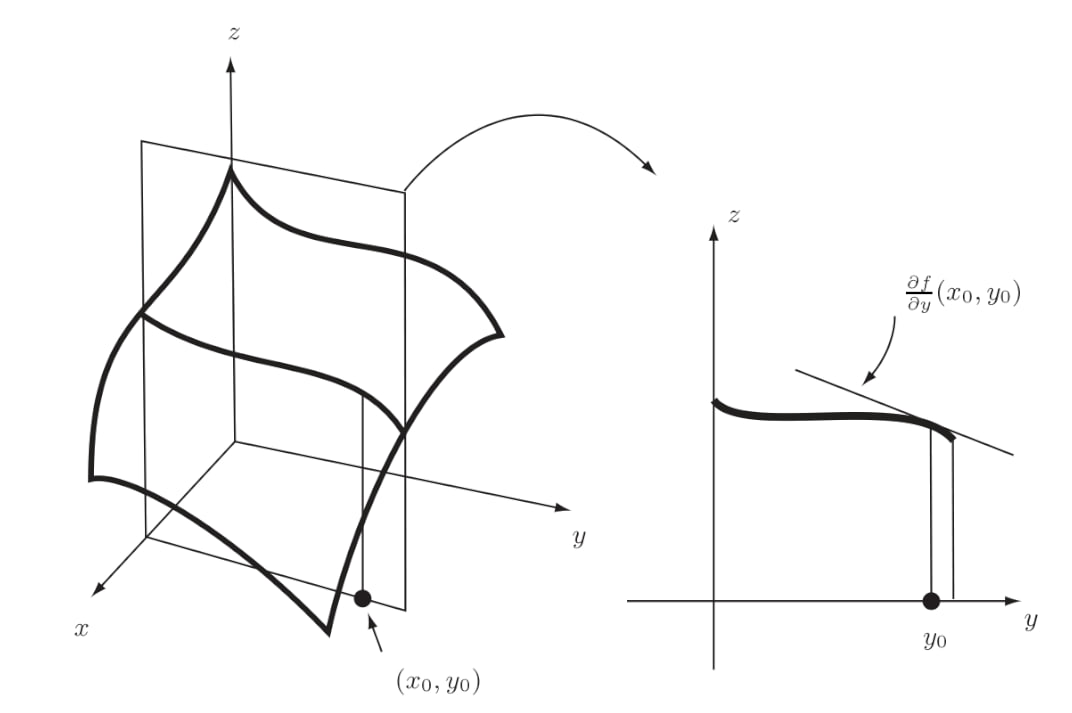
\includegraphics[scale = 0.6]{images/partial_deri.jpg}
    \caption{Мы рассекли график $z =f(x,y)$ плоскостью, параллельной плоскости $yz$, через точку $(x_0,y_0,0)$. Тогда мы получаем кривую, которая представляется какой-то функцией от $y$, и её наклон и есть $\frac{\partial f}{\partial y}(x_0,y_0)$.}
    \label{fig:enter-label}
\end{figure}

С другой стороны, мы можем пойти дальше и рассечь этот же график, но уже не параллельной ни плоскости $yz$, ни плоскости $xz$. Как тогда вычислить наклон?
5
\begin{figure}[h!]
    \centering
    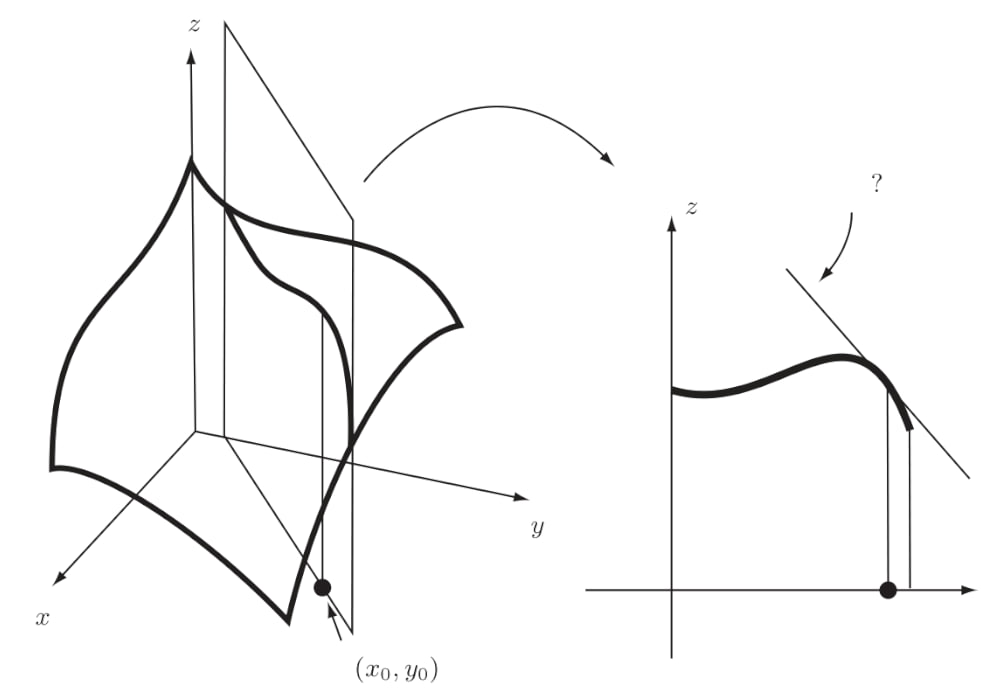
\includegraphics[scale=0.6]{images/direction_der.jpg}
    \caption{Мы рассекли график плоскостью, но уже не параллельной ни плоскости $yz$, ни плоскости $xz$.}
    \label{fig:enter-label}
\end{figure}

Чтобы ответить на этот вопрос, мы рассмотрим множество всех прямых, которые касаются графика в точке $(x_0, y_0, f(x_0,y_0))$. Такое множество мы называем \textit{касательной плоскостью} к графику $z = f(x,y).$

\begin{figure}[h!]
    \centering
    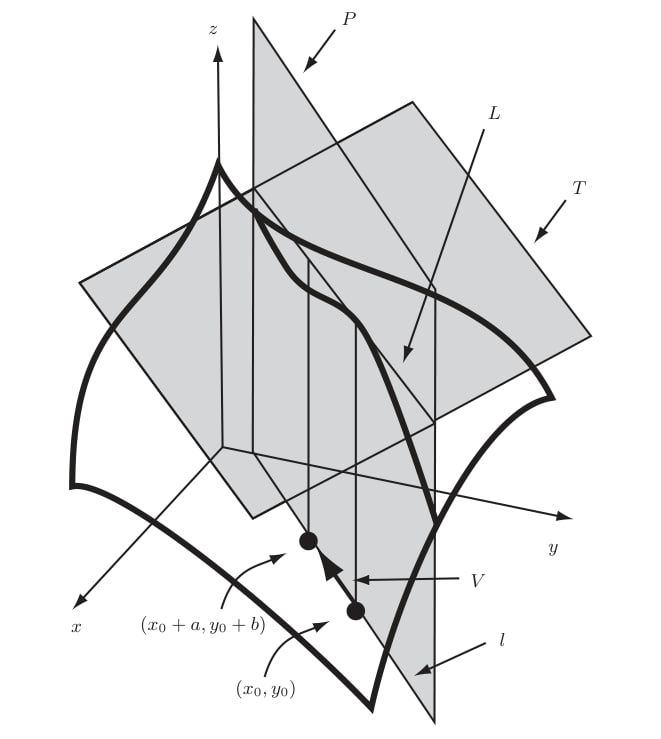
\includegraphics[scale =0.7]{images/direction_der2.jpg}
    \caption{Caption}
    \label{fig:enter-label}
\end{figure}

Уравнение плоскости, которая проходит через точку $(0,0,0)$, имеет вид $z = Ax + By$. Тогда сдвинув эту плоскость к точке $(x_0, y_0, f(x_0,y_0))$, мы получим тогда такое уравнение плоскости: $z - f(x_0,y_0) = A(x-x_0) + B(y-y_0)$. Осталось найти коэффициенты $A,B$, чтобы эта плоскость стала касательной. Пересечём эту плоскость с плоскостью $y=y_0$, в результате мы получаем прямую $z(x, y_0) - f(x_0,y_0) = A(x-x_0)$, тогда потребовав, чтобы эта прямая была касательной, мы получаем, что $A = \frac{\partial f}{\partial x}(x_0,y_0)$. Аналогично находим $B = \frac{\partial f}{\partial y}(x_0,y_0)$.

Итак, уравнение плоскости имеет вид
\[
z - f(x_0,y_0) = \left.\frac{\partial f}{\partial x}\right|_{(x_0,y_0)} (x-x_0) + \left.\frac{\partial f}{\partial y}\right|_{(x_0,y_0)} (y-y_0)
\]

Вернёмся ещё раз к предыдущему рисунку. Введём обозначения. Пусть $P$ -- вертикальная плоскость, проходящая через точку $(x_0,y_0)$. Пусть $\ell$ -- прямая, по которой $P$ пересекает плоскость $xy$. Касательную прямую к кривой, которую высекает плоскость $P$, мы обозначим через $L$. Касательная плоскость в точке $(x_0,y_0, f(x_0,y_0))$ пусть будет $T$. Далее, рассмотрим вектор $\m{v}$, который лежит на $\ell$, выходит из точки $(x_0,y_0)$ и кончается в $(x_0+a, y_0 +b)$, \ie имеет координаты $(a,b)$.

Имеем
\begin{eqnarray*}
    T(x_0 + a, y_0 + b) - T(x_0,y_0) &=& \left.\frac{\partial f}{\partial x}\right|_{(x_0,y_0)} (x_0 +a-x_0) + \left.\frac{\partial f}{\partial y}\right|_{(x_0,y_0)} (y_0 +b-y_0) \\
    &=& a\left.\frac{\partial f}{\partial x}\right|_{(x_0,y_0)} + b\left.\frac{\partial f}{\partial y}\right|_{(x_0,y_0)} \\
    &=& \langle \m{v} , \nabla f (x_0, y_0) \rangle
\end{eqnarray*}

Тогда, чтобы вычислить наклон, нужно потребовать, чтобы один из катетов в прямоугольном треугольнике был равен $1$, таким образом, если $a^2 + b^2 = 1$, то искомый наклон и есть число $\langle \m{v} , \nabla f (x_0, y_0) \rangle.$

\begin{definition}
    Пусть $\gamma: (-c,c) \to \mathbb{R}^n$ -- кривая в $\mathbb{R}$, \ie отображение непрерывно. Пусть $\gamma(0) = \m{x}_0$, и пусть $\gamma$ дифференцируема в точке $t = 0$, и $\dot\gamma(0) = \m{v}.$ Наконец, пусть $f:\mathbb{R}^n \to \mathbb{R}$ -- дифференцируемая в точке $\m{x}_0$ функция, тогда число 
    \[
     \nabla_{\dot\gamma(0)}(f):= \dfrac{1}{||\dot\gamma(0)||}\langle \nabla f(\m{x}_0), \dot\gamma(0) \rangle
    \]
    называется \textit{производной по направлению функции $f$ вдоль вектора $\dot \gamma(0)$.}
\end{definition}


Более проще, производную по направлению можно определить следующим образом
\begin{definition}
    Пусть дана точка $\m{p} \in \mathbb{R}^n$, вектор $\m{v}\in \mathbb{R}^n$ и пусть $f:\mathbb{R}^n \to \mathbb{R}$ -- функция. Тогда \textit{производная по направлению $\m{v}$ вычисленная в точке $\m{p}$} есть выражение вида
    \[
     (\nabla_\m{v}f)(\m{p}): = \frac{1}{\| \m{v}\|} (\mathrm{d}f)_\m{p} \m{v},
    \]
\end{definition}
где справа стоит умножение матриц. А именно, так как
\[
 (\mathrm{d}f)_\m{p} = \begin{pmatrix}
     f'_{x_1}(\m{p}) & \ldots & f'_{x_n}(\m{p})
 \end{pmatrix} \in \mathrm{Mat}_{1\times n}(\mathbb{R}),
\]
то получаем
\[
 \boxed{
 (\nabla_\m{v}f)(\m{p}) =\frac{1}{\|\m{v}\|} \left(  f'_{x_1}(\m{p})v_1 + \cdots + f'_{x_n}(\m{p}) v_n\right).
 }
\]



Рассмотрим теперь отображение $F: \mathbb{R}^n \to \mathbb{R}^m$, которое задаётся следующим образом:
\[
 F: \begin{pmatrix}
      x_1 \\ \vdots \\ x_n
 \end{pmatrix} \mapsto 
 \begin{pmatrix}
     f_1(x_1, \ldots, x_n) \\ \vdots \\ f_m(x_1, \ldots, x_n),
 \end{pmatrix}
\]
где $f_i:\mathbb{R}^n \to \mathbb{R}$. Потребуем, чтобы $F$ была дифференцируема в каком-то открытом $\mathscr{U} \subseteq \mathbb{R}^n$ или в фиксированной точке $\m{x}_0$. 

Тогда 
\[
 F(\m{x} + \m{h}) - F(\m{h}) = (\mathrm{d}_\m{x}F)(\m{h}) + o(||\m{h}||).
\]

Пусть $\m{h} = h_i \m{e}_i$, тогда $(\mathrm{d}_\m{x}F)(\m{e}_i)$ есть $i$-ый столбец матрицы $(\mathrm{d}_\m{x}F)(\m{h})$, и мы получаем равенство
\[
 \begin{pmatrix}
     f_1(x_1, \ldots, x_i + h_i, \ldots, x_n) -f_1(x_1, \ldots, x_i, \ldots, x_n) \\
     \vdots \\
     f_m(x_1, \ldots, x_i + h_i, \ldots, x_n) -f_m(x_1, \ldots, x_i, \ldots, x_n)
 \end{pmatrix} = h_i(\mathrm{d}_\m{x}F)(\m{e}_i) + o(|h_i|), \qquad 1 \le i \le n
\]
тогда
\[
 (\m{d}F)_\m{x}(\m{e}_i) = \begin{pmatrix}
     \frac{\partial f_1}{\partial x_i} \\ \vdots \\ \frac{\partial f_m}{\partial x_i}
 \end{pmatrix}
\]
и в итоге
\[
 (\m{d}F)_\m{x} = \begin{pmatrix}
     \frac{\partial f_1}{\partial x_1} & \ldots & \frac{\partial f_1}{\partial x_n} \\
     \vdots & \ddots & \vdots \\
     \frac{\partial f_m}{\partial x_1} & \ldots & \frac{\partial f_m}{\partial x_n}
 \end{pmatrix}, \qquad 
 (\m{d}F)_{\m{x}_0} = \begin{pmatrix}
     \frac{\partial f_1}{\partial x_1}({\m{x}_0}) & \ldots & \frac{\partial f_1}{\partial x_n} ({\m{x}_0}) \\
     \vdots & \ddots & \vdots \\
     \frac{\partial f_m}{\partial x_1} ({\m{x}_0}) & \ldots & \frac{\partial f_m}{\partial x_n} ({\m{x}_0})
     \end{pmatrix}
    \]

Такая матрица называется \textit{матрицей Якоби} отображения $F.$



\section{Необходимые и достаточные условия дифференцируемости}

Что касается необходимых условия дифференцируемости, то мы их уже знаем. Но для удобства мы сделаем из этого следующую теорему:

\begin{theorem}
    Если функция $f:\mathbb{R}^n \to \mathbb{R}$ дифференцируема на каком-то открытом $\mathscr{U} \subseteq \mathbb{R}^n$ или в фиксированной точке $\m{x}$, то она имеет в этой точке частные производные по всем переменным.
\end{theorem}

\begin{proof}
   Пусть $f:\mathbb{R}^n \to \mathbb{R}$, дифференцируемая на каком-то открытом $\mathscr{U} \subseteq \mathbb{R}^n$ или в фиксированной точке $\m{x}$. Тогда её дифференциал $(\mathrm{d}f)_\m{x}$ в точке $\m{x}$ задаётся матрицей размера $n\times 1$, $(\mathrm{d}f)_\m{x} = \begin{pmatrix}
    a_1 & \ldots & a_n
\end{pmatrix}$, где все $a_i$ есть функции от $\m{x}$. Наша цель -- найти эти $a_i$. Пусть $\m{h} = (h_1, \ldots, h_n)^\top \in \mathscr{U} \subseteq \mathbb{R}^n$, тогда получаем
\begin{eqnarray*}
    f(\m{x} + \m{h}) - f(\m{x}) &=& (\mathrm{d}f)_\m{x}(\m{h}) + o(||\m{h}||) \\
    &=& \begin{pmatrix}
        a_1 & \ldots & a_n
    \end{pmatrix} \begin{pmatrix}
        h_1 \\ \vdots \\ h_n  \end{pmatrix} + o(||\m{h}||) \\
        &=& a_1h_1 + \cdots + a_nh_n + o(||\m{h}||).
\end{eqnarray*}

Видно, что $a_i$ не зависит от координат вектора $\m{h}$ кроме $h_i$ \ie чтобы найти $a_i$, нам достаточно рассмотреть вектор $\m{h}_i = h_i \m{e}_i$, где $\m{e}_i$ -- базисный вектор. В таком случае, $||\m{h}_i|| = |h_i|$, и тогда для каждого $1 \le i \le n$ мы получаем
\[
 f(\m{x} + h_i \m{e}_i) - f(\m{x}) = a_ih_i + o(|h_i|),
\]
таким образом, 
\[
 a_i = \lim_{h_i \to 0} \frac{f(\m{x} + h_i \m{e}_i) - f(\m{x})}{h_i},
\]
такое выражение называется \textit{частной производной функции по переменной $x_i$} и обозначается либо как $\frac{\partial f}{\partial x_i}$, либо как $f'_{x_i}$, \ie 
\[
 \frac{\partial f}{\partial x_i}: = \lim_{h_i \to 0} \frac{f(\m{x} + h_i \m{e}_i) - f(\m{x})}{h_i},
\]
если же мы хотим знать её значение в точке $\m{x}_0$, то получаем
\[
 \frac{\partial f}{\partial x_i}(\m{x}_0): = \lim_{h_i \to 0} \frac{f(\m{x}_0 + h_i \m{e}_i) - f(\m{x}_0)}{h_i}.
\]
\end{proof}


Таким образом, в случае функции $f:\mathbb{R}^n \to \mathbb{R}$, дифференциал в точке $\m{x}_0$ находится по формуле
\[
 (\mathrm{d}f)_{\m{x}_0}: = \begin{pmatrix}
     \frac{\partial f}{\partial x_1}(\m{x}_0) & \ldots & \frac{\partial f}{\partial x_n}(\m{x}_0)
 \end{pmatrix}.
\]



Мы сейчас обобщим теорему Лагранжа о конечных приращениях. Ради краткости мы будем говорить, что вектор $\m{v} = (v_1,\ldots, v_n)^\top$ \textit{лежит между нулём и вектором} $\m{h} = (h_1,\ldots, h_n)^\top$, если $0\le v_i \le h_i$. $1\le i \le n.$

\begin{theorem}[Формула конечных приращений]\label{gen_of_Langrange}
    Пусть $\mathscr{U} \subseteq \mathbb{R}^n$ -- открытое множество, $f:\mathscr{U} \to \mathbb{R}$ -- функция, у которой во всех точках множества $\mathscr{U}$ имеются конечные частные производные по всем переменным. Тогда для любых $\m{a}, \m{a} + \m{h} \in \mathscr{U}$ справедливо равенство
\[
 f(\m{a} + \m{h}) - f(\m{a}) = \sum_{k =1}^n f'_{x_k}({\m{a} + \m{v}_k}) \cdot h_k,
\]
где $\m{v}_1, \ldots, \m{v}_n$ -- некоторые векторы, расположенные между нулём и вектором $\m{h}.$
\end{theorem}

\begin{proof}
    Пусть
\[
\begin{matrix}
     f_1 & = & f(a_1 + h_1, a_2, \ldots, a_n) - f(a_1, \ldots, a_n), \\
     f_2 & = & f(a_1 + h_1, a_2+h_2,a_3 \ldots, a_n) - f(a_1+h_1, \ldots, a_n),\\
     f_3 &=& f(a_1+h_1, a_2+h_2, a_3+h_3,a_4,\ldots, a_n) - (a_1 + h_1, a_2+h_2,a_3 \ldots, a_n),\\
     \vdots &  & \vdots \\
     f_n & = & f(a_1 + h_1, \ldots, a_n+h_n) - f(a_1, \ldots, a_n),
\end{matrix}
\]
тогда $f(\m{a} + \m{h}) - f(\m{a}) = f_1 + \cdots + f_n.$

Пусть 
\[
 \varphi_k(t): = f(a_1 + h_1, \ldots, a_{k-1}+h_{k-1},a_k+t_k, a_{k+1}, \ldots, a_n) - f(a_1 + h_1, \ldots, a_{k-1}+h_{k-1}, a_k,\ldots, a_n).
\]

Для удобства мы запишем в векторном виде, \ie в таком виде
\[
 \varphi_k(t): = f(\m{a} + h_1 \m{e}_1 + \cdots + h_{k-1}\m{e}_{k-1} + t\m{e}_k) - f(\m{a} + h_1 \m{e}_1 + \cdots + h_{k-1}\m{e}_{k-1})
\]

Тогда получаем
\begin{eqnarray*}
    \varphi_k(t) - \varphi_k(t_0) &=& f(\m{a} + h_1 \m{e}_1 + \cdots + h_{k-1}\m{e}_{k-1} + t\m{e}_k) - f(\m{a} + h_1 \m{e}_1 + \cdots + h_{k-1}\m{e}_{k-1}) \\
    &-& -f(\m{a} + h_1 \m{e}_1 + \cdots + h_{k-1}\m{e}_{k-1} + t_0\m{e}_k) + f(\m{a} + h_1 \m{e}_1 + \cdots + h_{k-1}\m{e}_{k-1}) \\
    &=& f(\m{a} + h_1 \m{e}_1 + \cdots + h_{k-1}\m{e}_{k-1} + t\m{e}_k) - f(\m{a} + h_1 \m{e}_1 + \cdots + h_{k-1}\m{e}_{k-1} + t_0\m{e}_k),
\end{eqnarray*}
в частности
\[
 \varphi_k(h_k) - \varphi_k(0) = f_k.
\]

Пусть $\m{x}_0 := \m{a}+ h_1 \m{e}_1 + \cdots + h_{k-1}\m{e}_{k-1}+t_0\m{e}_k$, тогда 
\begin{eqnarray*}
    \m{a} + h_1 \m{e}_1 + \cdots + h_{k-1}\m{e}_{k-1} + t\m{e}_k &=& \m{a} + h_1 \m{e}_1 + \cdots + h_{k-1}\m{e}_{k-1} + (t-t_0)\m{e}_k \\
    &+& \m{a} + h_1 \m{e}_1 + \cdots + h_{k-1}\m{e}_{k-1} + t_0\m{e}_k \\
    &=& \m{x}_0 + (t-t_0) \m{e}_k
\end{eqnarray*}

Таким образом, мы можем написать
\begin{eqnarray*}
    \varphi_k(t) - \varphi_k(t_0) &=&  f(\m{a} + h_1 \m{e}_1 + \cdots + h_{k-1}\m{e}_{k-1} + t\m{e}_k) - f(\m{a} + h_1 \m{e}_1 + \cdots + h_{k-1}\m{e}_{k-1} + t_0\m{e}_k) \\
    &=& f(\m{x}_0 + (t-t_0) \m{e}_k) - f(\m{x}_0),
\end{eqnarray*}
а тогда
\begin{eqnarray*}
    \varphi_k'(t_0) &:=& \lim_{t \to t_0} \frac{\varphi_k(t) - \varphi_k(t_0)}{t-t_0} \\
    &=& \lim_{t \to t_0} \frac{f(\m{x}_0 + (t-t_0) \m{e}_k) - f(\m{x}_0)}{t-t_0} \\
    &=:& \left.\frac{\partial f}{\partial x_k}\right|_{\m{x}_0} = f'_{x_k}(\m{x}_0).
\end{eqnarray*}

Это значит, что функция $\varphi_k(t)$ дифференцируема на отрезке $[0,h_k]$, потому что по условию существуют все частные производные в $\mathscr{U}$. 

Применим теперь к каждой $\varphi_k(t)$ теорему Лагранжа (теорема \ref{Langrange}); существует $\theta_k \in (0, h_k)$ такое, что
\[
 \varphi_k'(\theta_k) = \frac{\varphi_k(h_k) - \varphi_k(0)}{h_k}, 
\]
тогда, если $\m{v}_k:= \m{a}+ h_1 \m{e}_1  + \cdots + h_{k-1}\m{e}_{k-1} + \theta_k\m{e}_k$, то для каждого $1\le k \le n$ мы получили
\[
 f_k = \varphi_k(h_k) - \varphi_k(0) = \varphi_k'(\theta_k)h_k = f'_{x_k}(\m{a} + \m{v}_k)h_k, 
\]
где все $\m{k}$ расположены между $\m{a}$ и $\m{a}+ \m{h}$, тогда окончательно получаем
\begin{eqnarray*}
    f(\m{a} + \m{h}) - f(\m{a}) &=& f_1 + \cdots + f_n \\
    &=& f'_{x_1}(\m{a} + \m{v}_1)h_1 + \cdots + f'_{x_n}(\m{a} + \m{v}_n)h_n \\
    &=& \sum_{k =1}^n f'_{x_k}({\m{a} + \m{v}_k}) \cdot h_k,
\end{eqnarray*}
что и требовалось доказать.
\end{proof}




\begin{theorem}[Достаточные условия дифференцируемости]
    Пусть функция $f$ имеет конечные частные производные по всем координатам в окрестности точки $\m{a}$. Если они непрерывны в точке $\m{a}$, то $f$ дифференцируема в этой точке.
\end{theorem}

\begin{proof}
    Пусть $\mathscr{U}$ -- окрестность точки $\m{a}$, и пусть $\m{a} + \m{h} \in \mathscr{U}$. Согласно формуле конечных приращений, (теорема \ref{gen_of_Langrange}) мы имеем
    \[
     f(\m{a} + \m{h}) - f(\m{a}) = \sum_{k=1}^n  f'_{x_k}({\m{a} + \m{v}_k})\cdot h_k,
    \]
    где $\m{a} + \m{v}_k \in \mathscr{U}$, $1 \le k \le n$.

    По условию, все частные производные непрерывны и конечны, тогда для любого $\varepsilon >0$ из $||\m{v}_k|| < \delta$ следует $|f'_{x_k}({\m{a} + \m{v}_k}) - f'_{x_k}(\m{a})| < \varepsilon$. Другими словами, можно сказать, что
    \[
     f'_{x_k}({\m{a} + \m{v}_k}) = f_{x_k}'(\m{a}) + \varepsilon_k(\m{h}),
    \]
    где $\varepsilon_k(\m{h}) \to 0$ когда $\m{h} \to 0.$

    Таким образом, получаем
    \[
    f(\m{a} + \m{h}) - f(\m{a}) = \sum_{k=1}^n \bigl( f'_{x_k}(\m{a}) + \varepsilon_k(\m{h})  \bigr)h_k = \sum_{k=1}^n f'_{x_k}(\m{a}) h_k + \alpha(\m{h}),
    \]
    где $\alpha(\m{h}): = \sum_{k=1}^n \varepsilon_k(\m{h}) h_k$. Ясно, что
    \[
     \frac{\alpha(\m{h})}{|| \m{h} ||} = \sum_{k=1}^n \varepsilon_k(\m{h}) \frac{h_k}{||\m{h} ||}.
    \]

Наконец, согласно (\ref{m<d<M}), 
\[
 || \m{h} || = \sqrt{h_1^2 + \cdots + h_n^2} \ge  \max_{1\le i \le n} |h_i|,
\]
тогда 
\[
\frac{h_k}{|| \m{h}||} < \frac{h_i}{ \max_{1\le i \le n} |h_i|} \le \frac{\max_{1\le i \le n} |h_i|}{\max_{1\le i \le n} |h_i|} = 1 
\]
\ie все дроби $\frac{h_k}{||\m{h}||}$ ограничены. Далее, так как $\varepsilon_k(\m{h})$ бесконечно малые, мы получаем
\[
  f(\m{a} + \m{h}) - f(\m{a}) = \sum_{k=1}^n f'_{x_k}(\m{a}) h_k + o(||\m{h}||),
\]
а это и означает, что $f$ дифференцируема.
\end{proof}

\section{Непрерывность линейных отображений}

Напомним, что линейное отображение $L: \mathbb{R}^n \to \mathbb{R}^m$ -- это такое отображение, что
\[
 L(\alpha \m{v} + \beta \m{u}) = \alpha L(\m{v}) + \beta L(\m{u}),
\]
для любых $\m{v}, \m{u} \in \mathbb{R}^n$, $\alpha,\beta \in \mathbb{R}$.

Заметим, что 
\[
 L(\m{0}_n) = \m{0}_m,
\]
где $\m{0}_k$ -- нулевой вектор векторного пространства $\mathbb{R}^k$.


\begin{definition}
    Говорят, что линейное отображение $L: \mathbb{R}^n \to \mathbb{R}^m$ ограничено, если существует такое $K \ge 0$, что для любого $\m{v} \in \mathbb{R}^n$, $|| L(\m{v}) || \le K ||\m{v}||.$
\end{definition}

\begin{proposition}\label{contous_of_linear}
    Пусть $L: \mathbb{R}^n \to \mathbb{R}^m$ -- линейное отображение. Тогда следующие утверждения равносильны:
    \begin{enumerate}
        \item $L$ -- непрерывно.
        \item $L$ -- непрерывно в нуле.
        \item Существует такое $C > 0$, что $|| L(\m{v})| \le C ||\m{v}||$ для любого $\m{v} \in \mathbb{R}^n$
    \end{enumerate}
\end{proposition}
\begin{proof}
(1) $\Longrightarrow$ (2). Это просто следует из того, что если $L$ непрерывно, то оно непрерывно во всех точках $\mathbb{R}$, в частности и в нуле тоже.

(2) $\Longrightarrow$ (3). Если $L$ непрерывно в нуле, то это значит, что для любого $\varepsilon >0$ можно всегда найти такое $\delta>0$, что из $||\m{h}|| <\delta$ будет следовать $||L(\m{h})|| <\varepsilon$. Пусть $\varepsilon = 1$, тогда мы всегда найдём такой $\delta>0$, что если $|| \m{h} || < \delta$, то $|| L(\m{h})|| < 1$. Зафиксируем такое $\delta.$

Возьмём теперь произвольный ненулевой вектор\footnote{Аксиома Выбора позволяет.} $\m{v}$, тогда имеем
\begin{eqnarray*}
 || L(\m{v}) || &=& \left\| \frac{2}{\delta} || \m{v} || L\left(  \frac{\delta \m{v}}{2 || \m{v} ||}\right) \right\| \\
 &=&  \frac{2}{\delta} || \m{v}|| \cdot \left\| L\left(  \frac{\delta \m{v}}{2 || \m{v} ||}\right) \right\| < \frac{2}{\delta} || \m{v}||
\end{eqnarray*}
потому что 
\[
 \left\|\frac{\delta \m{v}}{2 || \m{v} ||} \right\| = \frac{\delta}{2} < \delta,
\]
и так как $\delta$ фиксировано, мы получаем требуемое.

(3) $\Longrightarrow$ (1). Имеем
\[
 || L(\m{v}) - L(\m{u}) || = || L(\m{v} - \m{u}) || \le K || \m{u} - \m{v} ||,
\]
тогда если $||\m{u} - \m{v}|| < \delta$, то $|| L(\m{v}) - L(\m{u}) ||< K \delta$,
поэтому для любого $\varepsilon >0$, если мы положим, что $0<\delta < \frac{\varepsilon}{K}$, то мы и получаем непрерывность $L$.
\end{proof}




\begin{lemma}\label{linear_is_contious}
    Любое линейное отображение $L: \mathbb{R}^n \to \mathbb{R}^m$ непрерывно. 
\end{lemma}
\begin{proof}
Пусть $L$ задаётся матрицей $(a_{i,j})_{1\le i \le n, 1 \le j \le m}$, тогда

\[
 L(\m{v}) = \begin{pmatrix}
     a_{11} & \ldots & a_{1n} \\
     \vdots & \ddots & \vdots \\
     a_{m1} & \ldots & a_{mn}
 \end{pmatrix}   \begin{pmatrix}
     v_1 \\ \vdots \\ v_n
 \end{pmatrix} = \begin{pmatrix}
     a_{11}v_1 + \cdots + a_{1n}v_n \\
     \vdots \\
     a_{m1}v_1 + \cdots + a_{mn}v_n 
 \end{pmatrix} = (u_1, \ldots, u_m)^\top =:\m{u} \in \mathbb{R}^m,
\] 
тогда
\begin{eqnarray*}
    ||L(\m{v})|| &=& ||\m{u}|| \\
    &=& \sqrt{(a_{11}v_1 + \cdots + a_{1n}v_n)^2 + \cdots + (a_{m1}v_1 + \cdots + a_{mn}v_n)^2} \\
    &\le & \sqrt{ m } \max_{1 \le k \le m} \left| a_{k1}v_1 + \cdots + a_{kn}v_n  \right| \\
    &\le & \sqrt{ m } \max_{1 \le k \le m} \left( |a_{k1}| \cdot |v_1| + \cdots + |a_{kn}| \cdot |v_n| \right) \\
    &\le & \sqrt{ m } \max_{1 \le k \le m} \left(|a_{k1}| \cdot || \m{v}|| + \cdots + |a_{kn}| \cdot || \m{v}||  \right) \\
    &=& \sqrt{ m } \max_{1 \le k \le m}\left(|a_{k1}|  + \cdots + |a_{kn}|   \right) \cdot || \m{v}|| \\
    &=& K || \m{v}||,
\end{eqnarray*}
где $K: = \sqrt{ m } \max_{1 \le k \le m}\left(|a_{k1}|  + \cdots + |a_{kn}|   \right)$, тогда по Предложению \ref{contous_of_linear} оно непрерывно. 
\end{proof}

\section{Дифференциал композиции}




\begin{theorem}\label{d(FG)}
    Пусть $F: \mathbb{R}^n \to \mathbb{R}^k$ дифференцируема в $\m{a} \in \mathbb{R}^n$, $G: \mathbb{R}^k \to \mathbb{R}^m$ дифференцируемо в $\m{b}= F(\m{a})$. Тогда $H: = G \circ F :\mathbb{R}^n \to \mathbb{R}^m$ дифференцируемо в $\m{a}$ и 
    \[
     (\mathrm{d}H)_\m{a} = (\mathrm{d}G)_{\m{b}} \cdot (\mathrm{d}F)_\m{a},
    \]
    где подразумевается обычное умножение матриц.
\end{theorem}


\begin{proof}

 Так как отображения дифференцируемо, мы имеем
 \[
  F(\m{a} + \m{h}) - F(\m{a}) = (\mathrm{d}F)_\m{a}(\m{h}) + \alpha(\m{h}) \cdot || \m{h}||,
 \] 
 и
 \[
  G(F(\m{a}) + \m{v})) - G(F(\m{a})) = (\mathrm{d}G)_{F(\m{a})}(\m{v}) + \beta(\m{v}) ||\m{v}||
 \]
где $\lim_{\m{h} \to \m{0}_n} \alpha (\m{h}) = \m{0}_k$, $\lim_{\m{v} \to \m{0}_k} \beta (\m{v}) = \m{0}_m$.

Мы можем положить $\beta(\m{0}_k) = \m{0}_m$ или доопределить её таким образом, видно, что на равенства это не повлияет. Тем самым, $\beta$ может считаться непрерывной в $\m{0}_k$.

Пусть $\m{v}: = F(\m{a} + \m{h}) - F(\m{a})$, тогда $G(F(\m{a}) + \m{v})) - G(F(\m{a}) = G(F(\m{a}+\m{h})) -G(F(\m{a}))$. 

Имеем

\begin{eqnarray*}
    G(F(\m{a}+\m{h})) -G(F(\m{a})) &=& (\mathrm{d}G)_{F(\m{a})}\bigl(F(\m{a}+ \m{h}) - F(\m{a})\bigr)  \\
    &+& \beta\Bigl( F(\m{a} +\m{h}) - F(\m{a}) \Bigr) \cdot || F(\m{a} + \m{h}) - F(\m{a})|| \\
    &=& (\mathrm{d}G)_{F(\m{a})} \Bigl( (\mathrm{d}F)_\m{a}(\m{h}) + \alpha(\m{h}) \cdot || \m{h}||\Bigr) \\
    &+& \beta \Bigl(F(\m{a} + \m{h}) - F(\m{a})\Bigr) \cdot \Bigl\| (\mathrm{d}F)_\m{a}(\m{h}) + \alpha(\m{h}) \cdot || \m{h}|| \Bigr\|
\end{eqnarray*}
из-за линейности $(\mathrm{d}G)_{F(\m{a})}$ получаем
\begin{eqnarray*}
    G(F(\m{a}+\m{h})) -G(F(\m{a})) &=&\Bigl((\mathrm{d}G)_{F(\m{a})} \circ (\mathrm{d}F)_\m{a}\Bigr) (\m{h}) + (\mathrm{d}G)_{F(\m{a})}((\alpha(\m{h})) \cdot || \m{h}|| \\
    &+& \beta \Bigl(F(\m{a} + \m{h}) - F(\m{a}) \Bigr) \cdot \Bigl\| (\mathrm{d}F)_\m{a}(\m{h}) + \alpha(\m{h}) \cdot || \m{h}|| \Bigr\|     
\end{eqnarray*}
вынесем теперь $|| \m{h}||$, получаем
\begin{eqnarray*}
    G(F(\m{a}+\m{h})) -G(F(\m{a})) &=&\Bigl((\mathrm{d}G)_{F(\m{a})} \circ (\mathrm{d}F)_\m{a}\Bigr) (\m{h})\\
    &+&\left( (\mathrm{d}G)_{F(\m{a})}\bigl((\alpha(\m{h})\bigr) + \beta \Bigl(F(\m{a} + \m{h}) - F(\m{a}) \Bigr) \cdot \left\| \frac{(\mathrm{d}F)_\m{a}(\m{h})}{|| \m{h} ||} + \alpha(\m{h})  \right\| \right) || \m{h} ||.     
\end{eqnarray*}

Так как $(\mathrm{d}F)_\m{a}: \mathbb{R}^n \to \mathbb{R}^k$ линейно, то по Лемме \ref{linear_is_contious} и Предложению \ref{contous_of_linear} оно ограничено, то есть $|| (\mathrm{d}F)_\m{a})(\m{h}) || \le K ||\m{h}||$. Далее, так как $(\mathrm{d}G)_{F(\m{a})}: \mathbb{R}^k \to \mathbb{R}^m$ линейно, то по Лемме \ref{linear_is_contious} оно непрерывно, и так как мы положили, что $\beta$ непрерывна в $\m{0}_k$, тогда 
\begin{eqnarray*}
 \lim_{\m{h} \to \m{0}_n}(\mathrm{d}G)_{F(\m{a})}\bigl((\alpha(\m{h})\bigr) &=& (\mathrm{d}G)_{F(\m{a})}\bigl( \lim_{\m{h} \to \m{0}_n} (\alpha(\m{h})\bigr) = \m{0}_m,\\
 \lim_{\m{h} \to \m{0}_n} \beta \Bigl(F(\m{a} + \m{h}) - F(\m{a}) \Bigr) &=& \beta (\m{0}_k) = \beta(\m{0}_m). 
\end{eqnarray*}

Далее, 
\[
  \left\| \frac{(\mathrm{d}F)_\m{a}(\m{h})}{|| \m{h} ||} + \alpha(\m{h})  \right\| \le \left\| \frac{(\mathrm{d}F)_\m{a}(\m{h})}{|| \m{h} ||} \right\| + \| \alpha(\m{h}) \| \le K + \| \alpha(\m{h}) \|,
\]
так как $\lim_{\m{h} \to \m{0}_n}\alpha(\m{h}) = \m{0}_k$, то согласно Предложению \ref{xn->x=||xn||->||x||}, Теореме \ref{f<g=>lim}:
\[
 0 \le \lim_{\m{h} \to \m{0}_n}\left\| \frac{(\mathrm{d}F)_\m{a}(\m{h})}{|| \m{h} ||} + \alpha(\m{h})  \right\| =C \le K.
\]

Итак, пусть
\[
 \omega (\m{h}): = \lim_{\m{h} \to \m{0}_n}\left( (\mathrm{d}G)_{F(\m{a})}\bigl((\alpha(\m{h})\bigr) + \beta \Bigl(F(\m{a} + \m{h}) - F(\m{a}) \Bigr) \cdot \left\| \frac{(\mathrm{d}F)_\m{a}(\m{h})}{|| \m{h} ||} + \alpha(\m{h})  \right\| \right),
\]
тогда мы показали, что
\[
 \lim_{\m{h} \to \m{0}_n} \omega (\m{h}) = \m{0}_m. 
\]

Окончательно мы получили, что
\[
 G(F(\m{a}+\m{h})) -G(F(\m{a})) =\Bigl((\mathrm{d}G)_{F(\m{a})} \circ (\mathrm{d}F)_\m{a}\Bigr) (\m{h}) +   \omega (\m{h}) || \m{h} ||,
\]
что и доказывает утверждение.
\end{proof}


\section{Дифференциалы высокого порядка}

Пусть дана функция $f: \mathbb{R}^n \to \mathbb{R}$ такая, что в открытом $\mathscr{U}$ у неё существуют все её частные производные $f_{x_i}' = \frac{\partial f}{\partial x_i}$. Пусть далее $\mathscr{V} \subseteq \mathscr{U}$ открыто, и пусть всюду в $\mathscr{V}$ её частные производные дифференцируемы, тогда мы получаем:
\begin{definition}
    Частные производные высокого порядка определяются как частные производные от частных производных, \ie
    \begin{eqnarray*}
        \frac{\partial^2 f}{\partial x_i \partial x_j} &:=& \frac{\partial }{\partial x_i}\left( \frac{\partial f}{\partial x_j} \right) = (f_{x_j}')'_{x_i} =: f''_{x_ix_j}. 
    \end{eqnarray*}
\end{definition}

\begin{mydanger}{\bf{!}}
    Выражение (если оно имеет смысл) 
    \[
     \frac{\partial f}{\partial x_i \partial x_j}
    \]
    называется \textit{смешанной производной}.
\end{mydanger}

\begin{theorem}[Шварц]
    Пусть $f:\mathbb{R}^2 \to \mathbb{R}$ имеет в окрестности $\mathscr{U}$ точки $\m{a} \in \mathbb{R}^2$ смешанные производные. Если эти производные непрерывны в этой точке, то они равны в этой точке, \ie
    \[
    \left.\frac{\partial f}{\partial x \partial y}\right|_\m{a} = \left.\frac{\partial f}{\partial y \partial x}\right|_\m{a}.
    \]
\end{theorem}

\begin{proof}
    Пусть $\m{a} = (a_1,a_2)^\top$, тогда, по определению (\ref{partial_i(o)}),
    \begin{eqnarray*}
       \left. \frac{\partial^2 f}{\partial x \partial y}\right|_\m{a} &=& \left. \frac{\partial}{\partial x}\left( \frac{\partial f}{\partial y} \right) \right|_\m{a} \\
       &=& \lim_{t \to 0} \left( \frac{\frac{\partial f}{\partial y}(a_1+t, a_2) - \frac{\partial f}{\partial y}(a_1,a_2)  }{t}  \right) \\
       &=& \lim_{t \to 0}\left( \frac{ \lim\limits_{s\to 0} \dfrac{f(a_1+t, a_2 +s) -f(a_1+t,a_2)}{s}  - \lim\limits_{s\to 0} \dfrac{f(a_1,a_2+s) -f(a_1,a_2)}{s} } {t}  \right) \\
       &=& \lim_{t\to 0} \lim_{s \to 0} \dfrac{f(a_1+t, a_2 +s) -f(a_1+t,a_2) - f(a_1,a_2+s) +f(a_1,a_2)}{ts} \\
       &=&\lim_{t\to 0} \lim_{s \to 0} \frac{\Phi(t,s)}{ts},
    \end{eqnarray*}
    где 
    \[
     \Phi(t,s):= f(a_1+t, a_2 +s) -f(a_1+t,a_2) - f(a_1,a_2+s) +f(a_1,a_2).
    \]

Аналогично, получаем
\[
 \left. \frac{\partial^2 f}{\partial y \partial x}\right|_\m{a} =  \lim_{s\to 0} \lim_{t \to 0} \frac{\Phi(t,s)}{ts}.
\]

Пусть 
\begin{eqnarray*}
 u(\tau) &: =& f(a_1 + \tau, a_2 + s) - f(a_1+ \tau, a_2), \qquad (a_1 + \tau, a_2) \in \mathscr{U} ,\\
 v(\sigma) &: =& f(a_1 + t, a_2 + \sigma) - f(a_1, a_2+\sigma), \qquad (a_1, a_2+\sigma) \in \mathscr{U} ,
\end{eqnarray*}

тогда
\[
 \Phi(t,s) = u(t) - u(0) = v(s) - v(0).
\]

Далее, так как по условию, $f$ имеет смешанные производные, значит она имеет и частные производные, а это значит, что $u(\tau)$, $v(\sigma)$ -- дифференцируемы на отрезках $[0,t]$ и $[0,s]$, соответственно. Тогда, по теореме Лагранжа \ref{Langrange} найдутся такие $\tau_0 \in (0, t)$ и $\sigma_0 \in (0, s)$, что
\begin{eqnarray*}
    \Phi(t,s) &=& u(t) - u(0) = u'(\tau_0)t,\\
    \Phi(t,s) &=& v(s) - v(0) = v'(\sigma_0)s.
\end{eqnarray*}

С другой стороны, 
\begin{eqnarray*}
    u'(\tau_0) &=& \frac{\partial}{ \partial x}\Bigl( f(a_1 + \tau_0, a_2 + s) - f(a_1+ \tau_0, a_2)\Bigr) \\
    &=& f'_x(a_1 + \tau_0, a_2 + s) - f'_x(a_1+ \tau_0, a_2).
\end{eqnarray*}

Аналогично, находим
\begin{eqnarray*}
    v'(\sigma_0) &=& \frac{\partial}{ \partial y}\Bigl( f(a_1+t, a_2 + \sigma_0) - f(a_1, a_2+\sigma_0)\Bigr) \\
    &=& f'_y(a_1 + t, a_2 + \sigma_0) - f'_x(a_1, a_2+\sigma_0).
\end{eqnarray*}

Пусть теперь
\begin{eqnarray*}
    w(\alpha) &:=& f'_y(a_1 + \alpha, a_2 + \sigma_0), \qquad 0 \le \alpha \le t \\
    g(\beta) &: =& f'_x(a_1 + \tau_0, a_2 + \beta), \qquad 0 \le \beta \le s.
\end{eqnarray*}

Тогда
\begin{eqnarray*}
    w(t)- w(0) &=& f'_y(a_1 + t, a_2 + \sigma_0) - f'_x(a_1, a_2+\sigma_0)= v'(\sigma_0),\\
    g(s) - g(0) &=& f'_x(a_1 + \tau_0, a_2 + s) - f'_x(a_1+ \tau_0, a_2) = u'(\tau_0).
\end{eqnarray*}

По условию, $f$ имеет смешанные частные производные на $\mathscr{U}$, тогда это значит, что $w$ и $g$ дифференцируемы на отрезках $[0,t]$ и $[0,s]$ соответственно. Тогда по теореме Лагранжа \ref{Langrange}, существуют такие $\alpha_0 \in (0,t)$ и $\beta_0 \in (0,s)$, что
\begin{eqnarray*}
    w(t)- w(0) &=& w'(\alpha_0) t = f''_{xy}(a_1+\alpha_0, a_2+\sigma_0)ts,\\
    g(s) -g(0) &=& g'(\beta_0)s = f''_{yx}(a_1 + \tau_0,a_2+\beta_0)ts.
\end{eqnarray*}

Таким образом, получаем
\begin{eqnarray*}
    \Phi(t,s) &=& u'(\tau_0)t \\
             &=& (g(s) - g(0))t \\
             &=& g'(\beta_0)ts \\
             &=& f''_{yx}(a_1 + \tau_0,a_2+\beta_0)st
\end{eqnarray*}
и
\begin{eqnarray*}
\Phi(t,s) &=& v'(\sigma_0)s \\
             &=& (w(t) - w(0))s \\
             &=& w'(\alpha_0)st \\
             &=& f''_{xy}(a_1 + \alpha_0,a_2+\sigma_0)st.
\end{eqnarray*}

Ясно, что если $t,s \to 0$ то и $\alpha_0, \beta_0, \tau_0, \sigma_0 \to 0$, но тогда из-за предположения о непрерывности смешанных производных получаем
\begin{eqnarray*}
    \lim_{t\to 0} \lim_{s \to 0} \frac{\Phi(t,s)}{ts} &=&  \lim_{t\to 0} \lim_{s \to 0} f''_{xy}(a_1 + \alpha_0,a_2+\sigma_0) \\
    &=& \lim_{t \to 0} f''_{xy}(a_1 + \alpha_0,a_2) \\
    &=& f''_{xy}(a_1,a_2),
\end{eqnarray*}
и
\begin{eqnarray*}
    \lim_{s\to 0} \lim_{t \to 0} \frac{\Phi(t,s)}{ts} &=& \lim_{s\to 0} \lim_{t \to 0}f''_{yx}(a_1 + \tau_0,a_2+\beta_0)\\
    &=& \lim_{s\to 0}f''_{yx}(a_1,a_2+\beta_0) \\
    &=& f''_{yx}(a_1,a_2),
\end{eqnarray*}
что и доказывает утверждение.     
\end{proof}


\begin{theorem}[Юнг]\label{Yong}
    Пусть у функции $f:\mathbb{R}^2 \to \mathbb{R}$ в окрестности в точке $\m{a} = (a_1,a_2)^\top$ существуют частные производные $f'_{x}$ и $f'_{y}$. Если эти частные производные дифференцируемы в точке $\m{a}$, то
    \[
     f''_{xy}(a_1,a_2) = f''_{yx}(a_1,a_2).
    \]
\end{theorem}

%Нужно сказать про отличие от предыдущей.

\begin{proof}
    Сохраним те же обозначения, как и в доказательстве предыдущей теоремы и рассмотрим 
        \[
     \Phi(t,t):= f(a_1+t, a_2 +t) -f(a_1+t,a_2) - f(a_1,a_2+t) +f(a_1,a_2).
    \]

Повторим те же рассуждения, что и в предыдущем доказательстве. 

Пусть 
\begin{eqnarray*}
 u(\tau) &: =& f(a_1 + \tau, a_2 + t) - f(a_1+ \tau, a_2), \qquad (a_1 + \tau, a_2) \in \mathscr{U} ,\\
 v(\tau) &: =& f(a_1 + t, a_2 + \tau) - f(a_1, a_2+\tau), \qquad (a_1, a_2+\sigma) \in \mathscr{U} ,
\end{eqnarray*}

тогда
\[
 \Phi(t,t) = u(t) - u(0) = v(t) - v(0).
\]

Далее, так как по условию $f$ имеет смешанные производные, значит, она имеет и частные производные, а это значит, что $u(\tau)$, $v(\tau)$  дифференцируемы на отрезке $[0,t]$. Тогда по теореме Лагранжа \ref{Langrange} найдётся такое $\tau_0 \in (0, t)$, что
\begin{eqnarray*}
    \Phi(t,t) &=& u(t) - u(0) = u'(\tau_0)t,\\
    \Phi(t,t) &=& v(t) - v(0) = v'(\tau_0)t.
\end{eqnarray*}

По условию $f'_x$, $f'_y$ дифференцируемы в окрестности точки $\m{a}$, тогда
\begin{eqnarray*}
    f'_x(\m{a} + \m{h}) &=& f'_x(\m{a}) + (\mathrm{d}f_x')_\m{a} \m{h} + o(\m{h}), \\
    f'_y(\m{a} + \m{h}) &=& f'_y(\m{a}) + (\mathrm{d}f_y')_\m{a} \m{h} + o(\m{h}),
\end{eqnarray*}
при $\m{h} \to \m{0}.$

Тогда получаем
\begin{eqnarray*}
    u'(\tau_0) &=& f'_x(a_1 + \tau_0, a_2 + t) - f'_x(a_1+ \tau_0, a_2) \\
    &=& f'_x(a_1,a_2) + \begin{pmatrix}
        f''_{xx}(a_1,a_2) & f''_{xy}(a_1,a_2) 
    \end{pmatrix} \begin{pmatrix}
        \tau_0 \\ t
    \end{pmatrix} + \omega_1(\tau_0, s) \sqrt{\tau_0^2 +t^2} \\
    && - f_x'(a_1,a_2) - \begin{pmatrix}
        f''_{xx}(a_1,a_2) & f''_{xy}(a_1,a_2) 
    \end{pmatrix} \begin{pmatrix}
        \tau_0 \\ 0
    \end{pmatrix} - \omega_2(\tau_0, 0) \sqrt{\tau_0^2 +0^2} \\
    &=& f''_{xy}(a_1,a_2) t + \omega_1(\tau_0, t) \sqrt{\tau_0^2 +t^2}- \omega_2(\tau_0, 0) |\tau_0|.
\end{eqnarray*}

Аналогично, получаем
\begin{eqnarray*}
    v'(\tau_0) &=& f'_y(a_1 + t, a_2 + \tau_0) - f'_y(a_1, a_2+\tau_0) \\
    &=& f_y'(a_1, a_2) + \begin{pmatrix}
        f''_{yx}(a_1,a_2) & f''_{yy}(a_1,a_2) 
    \end{pmatrix} \begin{pmatrix} t\\ \tau_0
    \end{pmatrix} + \omega_3(t,\tau_0)\sqrt{t^2 +\tau_0^2} \\
    &&- f'_y(a_1,a_2) - \begin{pmatrix}
        f''_{yx}(a_1.a_2) & f''_{yy}(a_1,a_2)
    \end{pmatrix} \begin{pmatrix}
        0 \\ \tau_0
    \end{pmatrix} - \omega_4(0,\tau_0)|\tau_0| \\
    &=& f''_{yx}(a_1,a_2)t + \omega_3(t,\tau_0)\sqrt{t^2 +\tau_0^2} - \omega_4(0,\tau_0)|\tau_0|.
\end{eqnarray*}

Так как $\Phi(t,t) = u'(\tau_0)t = v'(\tau_0)t$, то мы получаем
\[
 \Bigl( f''_{xy}(a_1,a_2) t + \omega_1(\tau_0, t) \sqrt{\tau_0^2 +t^2}- \omega_2(\tau_0, 0) |\tau_0| \Bigr) t = \Bigl( f''_{yx}(a_1,a_2)t + \omega_3(t,\tau_0)\sqrt{t^2 +\tau_0^2} - \omega_4(0,\tau_0)|\tau_0| \Bigr)t,
\]
разделим обе части равенства на $t^2$
\[
  f''_{xy}(a_1,a_2) + \omega_1(\tau_0, t) \sqrt{1+ \left(\frac{\tau_0}{t}\right)^2}- \omega_2(\tau_0, 0) \frac{|\tau_0|}{t}=  f''_{yx}(a_1,a_2) + \omega_3(t,\sigma_0)\sqrt{1 +\left(\frac{\sigma_0}{t}\right)^2} - \omega_4(0,\sigma_0)\frac{|\sigma_0|}{t},
\]


Ввиду того, что $0 \tau_0 <t$, то $\sqrt{t^2 + (\frac{\tau_0}{t})^2}$, $\frac{\tau_0}{t}$ -- ограниченные функции, и так как $\omega_1, \omega_2, \omega_3, \omega_4 \in o(1)$ при $t \to 0$, мы получаем равенство
\[
  f''_{xy}(a_1,a_2) =  f''_{yx}(a_1,a_2),
\]
что и требовалось доказать.    
\end{proof}


\begin{definition}
    Пусть $f:\mathbb{R}^n \to \mathbb{R}$ -- дифференцируема в окрестности точки $\m{a}$. Говорят, что $f$ \textit{дважды дифференцируема в точке $\m{a}$}, если все её частные производные $f'_{x_i}$ дифференцируемы в точке $\m{a}$.

    Пусть $f$ -- $m$ раз дифференцируема в окрестности точки $\m{a}$. Говорят, что \textit{$f$ есть $m+1$ раз дифференцируемой в точке $\m{a}$}, если все частные производные $m$-го порядка $\frac{\partial^m f}{\partial x_{i_1} \cdots \partial x_{i_m}}$ дифференцируемы в точке $\m{a}$.
\end{definition}

\begin{corollary}\label{f''xy=f''yx}
    Если $f:\mathbb{R}^n \to \mathbb{R}$ есть $m$-раз дифференцируема в точке $\m{a}$, то значения производных порядка $m$ не зависят от порядка дифференцирования.
\end{corollary}

\begin{proof}
Это следует из теоремы Юнга \ref{Yong} с помощью индукции.


\end{proof}






\section{Высшие дифференциалы}

Рассмотрим дифференцируемое отображение $F: \mathbb{R}^n \to \mathbb{R}^m$ в каком-то открытом $\mathscr{U} \subseteq \mathbb{R}^n$, \ie для каждой точки $\m{p} \in \mathscr{U}$ у нас есть линейное отображение $(\mathrm{d}F)_{\m{p}}: \mathbb{R}^n\to \mathbb{R}^m$. Так как линейные отображения из $\mathbb{R}^n$ в $\mathbb{R}^m$ -- это просто матрицы размера $m\times n$, то дифференцируемость отображения $F$ в $\mathscr{U}$ означает, что у нас есть отображение
\[
 \mathrm{d}F: \mathscr{U} \to \mathrm{Mat}_{m\times n}(\mathbb{R}), \qquad \m{p} \mapsto (\mathrm{d}F)_{\m{p}}.
\]

С другой стороны, пространство матриц $\mathrm{Mat}_{m\times n}(\mathbb{R})$ есть векторное пространство, которое можно отождествить (=изоморфно) с $\mathbb{R}^{mn}$, \textit{т.е.,} мы имеем
\[
 \mathrm{d}F: \mathscr{U} \to \mathbb{R}^{mn}, \qquad \m{p} \mapsto (\mathrm{d}F)_{\m{p}}, \qquad \mathscr{U} \subseteq \mathbb{R}^n.
\]

Тогда мы можем поставить вопрос о дифференцируемости отображения $\mathrm{d}F$ и получить уже отображение
\[
 \mathrm{d}^2(F): = \mathrm{d}(\mathrm{d}F): \mathscr{U}' \to \mathrm{Mat}_{mn
 \times n}(\mathbb{R}),
\]
где $\mathscr{U}'$ открыто в $\mathscr{U}$.

Таким образом, мы получаем отображения (если они существуют)
\[
 F:=\mathrm{d}^0F,\quad  \mathrm{d}F,\quad \mathrm{d}^2(F): = \mathrm{d}(\mathrm{d}F), \ldots, 
\]
среди которых $\mathrm{d}^k(F)$ при $k>1$ называются \textit{высшими дифференциалами.}


\subsection{Явная формула для высших дифференциалов и формальный символизм}

Итак, пусть у нас есть $n$-раз дифференцируемая функция $f:\mathbb{R}^n \to \mathbb{R}$ в окрестности $\mathscr{U}$ точки $\m{a}$. Мы знаем, что
\[
 (\mathrm{d}f)_\m{a}(\m{h}) = \begin{pmatrix}
     f'_{x_1}(\m{a}) & \ldots & f'_{x_n}(\m{a})
 \end{pmatrix} \begin{pmatrix}
      h_1 \\ \vdots \\ h_n
 \end{pmatrix} = f_{x_1}'(\m{a})h_1 + \cdots + f_{x_n}'(\m{a})h_n.
\]

Найдём $(\mathrm{d}^n(f))_\m{a}(\m{h}): = \mathrm{d}(\mathrm{d}^{n-1}f)_\m{a}(\m{h})$. Для этого нам понадобиться следующий формализм.

Пусть $C^\infty(\mathbb{R}^n)$ есть множество гладких (=бесконечно дифференцируемых) дифференцируемых функций $f:\mathbb{R}^n \to \mathbb{R}$. Рассмотрим следующие отображения:
\[
 \frac{\partial}{\partial x_i}: C^\infty(\mathbb{R}^n) \to C^\infty(\mathbb{R}^n), \qquad f\mapsto f'_{x_i}, \quad 1 \le i \le n.
\]

Тогда у нас возникают их композиции 
\[
 \frac{\partial^k}{\partial x_{i_k} \cdots \partial x_{i_1}}:=\dfrac{\partial}{\partial x_{i_k}} \circ \cdots \circ \dfrac{\partial}{\partial x_{i_1}}:  C^\infty(\mathbb{R}^n) \to C^\infty(\mathbb{R}^n), \qquad f \mapsto \frac{\partial^k f}{\partial x_{i_k} \cdots \partial x_{i_1}}.
\]




\begin{theorem}\label{differential_formula}
    Если функция $f:\mathbb{R}^n \to \mathbb{R}$ в окрестности точки $\m{a}$ $m$ раз дифференцируема, то для каждого $1 \le k \le m$
    \[
     \boxed{
 (\mathrm{d}^kf)_\m{a}(\m{h})=     \left.\left(\frac{\partial}{\partial x_1} h_1 + \cdots + \frac{\partial }{\partial x_n}h_n \right)^k\right|_{\m{a}} \cdot f
    }\]
\end{theorem}
\begin{proof}
    Доказательство будет идти по индукции. Если $m=1$, то мы получаем просто определение дифференциала. Пусть формула верна при $1 \le k<m$, имеем
    \[
     (\mathrm{d}^kf)(\m{h}) = \sum_{p_1 + \ldots + p_n = k} \dfrac{k!}{p_1! \cdots p_n!} \frac{\partial^k f}{\partial x_1^{p_1} \cdots \partial x_n^{p_n}} h_1^{p_1}\cdots h_n^{p_n}
    \]

Дифференцируем теперь это равенство, получаем
\begin{eqnarray*}
    (\mathrm{d}^{k+1}f)(\m{h}) &=& (\mathrm{d}(\mathrm{d}^kf))(\m{h}) \\
     &=& \sum_{p_1 + \ldots + p_n = k} \dfrac{k!}{p_1! \cdots p_n!} \mathrm{d}\left( \frac{\partial^k f}{\partial x_1^{p_1} \cdots \partial x_n^{p_n}} h_1^{p_1}\cdots h_n^{p_n}\right) \m{h}\\
     &=& \sum_{p_1 + \ldots + p_n = k} \dfrac{k!}{p_1! \cdots p_n!} \left(\mathrm{d}\left( \frac{\partial^k f}{\partial x_1^{p_1} \cdots \partial x_n^{p_n}} \right)(\m{h}) \right)\cdot h_1^{p_1}\cdots h_n^{p_n} 
\end{eqnarray*}
    Теперь применяя формулу дифференциала, мы получим
\[
  (\mathrm{d}^{k+1}f)(\m{h}) = \sum_{p_1 + \ldots + p_n = k} \dfrac{k!}{p_1! \cdots p_n!} \left( \frac{\partial^{k+1}f}{\partial x_1^{p_1+1} \cdots \partial x_n^{p_n}}h_1 + \cdots +  \frac{\partial^{k+1}f}{\partial x_1^{p_1} \cdots \partial x_n^{p_n+1}}h_n \right)\cdot h_1^{p_1}\cdots h_n^{p_n}. 
\]

Фиксируем набор $(p_1,\ldots, p_n)$ и рассмотрим соответствующую сумму
\[
 S(p_1,\ldots, p_n): = \frac{\partial^{k+1}f}{\partial x_1^{p_1+1} \partial x_2^{p_2} \cdots \partial x_n^{p_n}}h_1^{p+1}h_2^{p_2}\cdots h_n^{p_n} + \cdots +  \frac{\partial^{k+1}f}{\partial x_1^{p_1} \cdots \partial x_n^{p_n+1}}h_1^{p_1}h_2^{p_2} \cdots h_n^{p_n+1}.
\]
тогда первое слагаемое этой суммы также присутствует в следующих суммах
\[
\begin{matrix}
    S(p_1+1, p_2-1,p_3,\ldots, p_n), \\
    S(p_1+1, p_2,p_3-1,\ldots, p_n), \\
    \vdots \\
    S(p_1+1, p_2,p_3,\ldots, p_n-1).
\end{matrix}
\]

Тогда коэффициент при $\frac{\partial^{k+1}f}{\partial x_1^{p+1}\partial x_2^{p_2} \cdots \partial x_n^{p_n}} h_1^{p_1+1}h_2^{p_2}\cdots h_n^{p_n}$ есть следующее выражение
\[
 K = \frac{k!}{p_1! p_2! \cdots p_n!} + \frac{k!}{(p_1+1)!(p_2-1)! \cdots p_n!} + \cdots + \frac{k!}{(p_1+1)!p_2! \cdots (p_n-1)!}
\]
имеем
\begin{eqnarray*}
  K &=&   \frac{k!}{p_1! p_2! \cdots p_n!} + \frac{k!}{(p_1+1)!(p_2-1)! \cdots p_n!} + \cdots + \frac{k!}{(p_1+1)!p_2! \cdots (p_n-1)!} \\
  &=& \frac{k!}{p_1! (p_2-1)! \cdots (p_n-1)!}\left( \frac{1}{p_2p_3 \cdots p_n} + \frac{1}{(p_1+1)p_2\cdots p_n} + \cdots + \frac{1}{(p_1+1)p_2 \cdots p_{n-1}}\right) \\
  &=& \frac{k!}{p_1! (p_2-1)! \cdots (p_n-1)!} \cdot \frac{p_1+1 +p_2+ \cdots+ p_n}{(p_1+1)p_2\cdots p_n} \\
  &=& \frac{k!(k+1)}{(p_1+1)! p_2! \cdots p_n!} \\
  &=& \frac{(k+1)!}{(p_1+1)! p_2! \cdots p_n!}.
\end{eqnarray*}

Таким образом, рассуждая аналогично для остальных мономов, мы можем тогда записать
\[
 (\mathrm{d}^{k+1}f)(\m{h}) = \sum_{p_1 + \ldots + p_n = k+1} \dfrac{(k+1)!}{p_1! \cdots p_n!} \frac{\partial^{k+1} f}{\partial x_1^{p_1} \cdots \partial x_n^{p_n}} h_1^{p_1}\cdots h_n^{p_n},
\]
что и доказывает утверждение.

\end{proof}


\section{Полином Тейлора от нескольких переменных}

Прежде всего рассмотрим следующую задачу. Пусть нам дана функция $\psi:\mathbb{R}^n \to \mathbb{R}$. Допустим что она дифференцируема в окрестности $\mathscr{U}$ точки $\m{a} = (a_1,\ldots, a_n)$, и пусть при $0\le t \le 1$, точка $\m{a}+t\m{h} = (a_1 + th_1, \ldots, a_n+th_n)$ также принадлежит этой же окрестности. Тогда, при фиксированных $\m{a}, \m{h}$ мы уже получаем функцию $\psi(\m{a}+t\m{h})$ от одной переменной. Как найти её производную?

\begin{lemma}
    Пусть $f:\mathbb{R}^n \to \mathbb{R}$ дифференцируема в окрестности точки $\mathscr{U}$ точки $\m{a}$, и пусть при $0\le t \le 1$, точка $\m{a}+t\m{h}\in \mathscr{U}$. Тогда, при фиксированных $\m{a}, \m{h}$, функция $\psi_{\m{a},\m{h}}(t):= f(\m{a}+t\m{h}):\mathbb{R} \to \mathbb{R}$ дифференцируема при $0 \le t \le 1$ и
    \[
     \psi_{\m{a},\m{h}}'(t) = \left.\frac{\partial f}{ \partial x_1}\right|_{\m{a} + t \m{h}} \cdot h_1 + \cdots + \left.\frac{\partial f}{ \partial x_n}\right|_{\m{a} + t \m{h}} \cdot h_n
    \]
\end{lemma}

\begin{proof}
Прежде всего мы видим, что наша функция $\psi_{\m{a},\m{h}}(t)$ есть композиция двух стрелок
\[
 \xymatrix{
 \mathbb{R} \ar@{->}[rr]^{t \mapsto \m{a}+ t\m{h}} \ar@{.>}[rd]_{t \mapsto \psi_{\m{a},\m{h}}(t)} && \mathbb{R}^n \ar@{->}[ld]^{\m{x} \mapsto \psi(\m{x})} \\
 & \mathbb{R} &
 }
\]

Далее, для функции от одной переменной, значение её производной это есть значение дифференциала вычисленного в этой же точке. Тогда по теореме о композиции \ref{d(FG)},
\[
 \psi'_{\m{a},\m{h}}(t) = (\mathrm{d}\psi)_t = (\mathrm{d}f)_{\m{a}+t\m{h}} \cdot (\mathrm{d}\gamma)_t,
\]
где 
\[
 \gamma(t): = \m{a}+t\m{h} = \begin{pmatrix}
     a_1 + th_1 \\ \vdots \\ a_n + t h_n
 \end{pmatrix}
\]
Тогда её матрица Якоби (=дифференциал) имеет вид
\[
 \mathrm{d}\gamma = \begin{pmatrix}
     \dot\gamma_1(t) \\ \vdots \\ \dot \gamma_n(t)
 \end{pmatrix} = \begin{pmatrix}
     h_1 \\ \vdots\\ h_n
 \end{pmatrix} = \m{h},
\]
здесь $\gamma_1(t) = a_1 + th_1,\ldots, \gamma_n(t) = a_n+th_n.$
Тогда, получаем
\begin{eqnarray*}
    \psi'_{\m{a},\m{h}}(t) & =& (\mathrm{d}\psi)_t = (\mathrm{d}f)_{\m{a}+t\m{h}} \cdot (\mathrm{d}\gamma)_t \\
    &=& (\mathrm{d}f)_{\m{a}+t\m{h}} \m{h} \\
    &=& \left.\frac{\partial f}{ \partial x_1}\right|_{\m{a} + t \m{h}} \cdot h_1 + \cdots + \left.\frac{\partial f}{ \partial x_n}\right|_{\m{a} + t \m{h}} \cdot h_n,
\end{eqnarray*}
что и требовалось доказать.
\end{proof}

\begin{corollary}\label{nice_nice}
    Если функция $f$ является $m$-раз дифференцируемое в точке $\m{a}$, то функция $\psi_{\m{a}, \m{h}}(t)$ является тоже $m$-раз дифференцируемой при $0\le t \le 1$, и более того 
    \[
     \psi_{\m{a},\m{h}}^{k}(t) = (\mathrm{d}^k_{\m{a}+t\m{h}}f)(\m{h}).
    \]
\end{corollary}

\begin{theorem}\label{Taylor_in_many}
    Пусть $f:\mathbb{R}^n \to \mathbb{R}$ есть $m+1$ раз дифференцируемая функция в окрестности точки $\m{a} \in \mathbb{R}^n$, то для всех $\m{h}$ из окрестности точки $\m{0}_n$ верно 
    \[
     f(\m{a} + \m{h}) = f(\m{a}) + (\mathrm{d}f)_\m{a} \m{h} + \frac{1}{2!} (\mathrm{d}^2f)_\m{a}\m{h} + \cdots + \frac{1}{m!} (\m{d}^mf)_\m{a}\m{h} + \frac{1}{(m+1)!} (\m{d}^{m+1}f)_{\m{a}+ \theta \m{h}}\m{h},
    \]
    где $0 < \theta < 1$ и она зависит от $\m{a}, \m{h}$ и $m$.
\end{theorem}
\begin{proof}
    Пусть $\varphi_{\m{a},\m{h}}(t): = f(\m{a}+t \m{h})$, $t \in [0,1]$, тогда согласно Следствию \ref{nice_nice}, она $m+1$ раз дифференцируема и более того 
    \[
     \varphi^{k}(t) = (\mathrm{d}^k_{\m{a}+t\m{h}}f)(\m{h}).
    \]

Тогда её полином Тейлора с остаточным мономом в форме Лагранже (Следствие \ref{monom_in_Langrange} имеет вид
\[
 \varphi(t) = \varphi(0) + \frac{\varphi'(0)}{1!}t + \frac{\varphi''(0)}{2!}t^2 + \cdots + \frac{\varphi^{(m)}(0)}{m!}t^m + \frac{\varphi^{(m+1)}(\theta)}{(m+1)!}t^{m+1}
\]
где $0 < \theta < t.$

Тогда, используя равенство 
 \[
     \varphi_{\m{a},\m{h}}^{k}(t) = (\mathrm{d}^k_{\m{a}+t\m{h}}f)(\m{h}), \qquad 1 \le k \le m+1.
    \]
    получаем
\begin{align*}
    &\varphi(0) = f(\m{a}), \\
    &\varphi^{(k)}(0) = (\mathrm{d}^k_{\m{a}}f)(\m{h}), \qquad 1 \le k \le m,\\
    &\varphi^{(m+1)}(\theta) =(\mathrm{d}^k_{\m{a}+\theta \m{h}}f)(\m{h}).
\end{align*}

Тогда мы можем записать
\[
 \varphi(t) = f(\m{a}) + \sum_{k=1}^m \frac{(\mathrm{d}^k_{\m{a}}f)(\m{h})}{k!}t^k + \frac{( \mathrm{d}^k_{\m{a}+\theta \m{h}}f)(\m{h}) }{(m+1)!}t^{m+1},
\]
так как $\varphi(1) = f(\m{a}+\m{h})$, то подставляя $t=1$ в последней сумме мы получаем требуемое.
 \end{proof}




\section{Компактные пространства}

Мы приступаем 

\begin{definition}
 Пусть $X$ -- произвольное непустое множество. Множество $(\mathscr{U}_\lambda)_{\lambda \in \Lambda}$ подмножеств множества $X$ называется его \textit{покрытием}, если $X = \bigcup_{\lambda \in \Lambda} \mathscr{U}_\lambda$.    
\end{definition}

Имеется и другое, более широкое понимание этих терминов: множество $(\mathscr{U}_\lambda)_{\lambda \in \Lambda}$ подмножеств множества $Y$ называется \textit{покрытием} множества $X\subseteq Y$, если $X \subseteq \bigcup_{\lambda \in \Lambda} U_\lambda$.


\begin{definition}
    Метрическое пространство $E$ называется \textit{компактным}, если оно удовлетворяет \boxed{\textbf{аксиоме Бореля -- Лебега)}}: для каждого покрытия $(\mathscr{U}_\lambda)_{\lambda \in \Lambda}$ пространства $E$ открытыми множествами (=открытое покрытие) существует конечное подсемейство $(\mathscr{U}_\lambda)_{\lambda \in L}$ (где $L \subseteq \Lambda$, и $L$ -- конечное множество), являющееся покрытием пространства $E.$
\end{definition}

\begin{definition}
\textit{Компактом} (или компактным множеством) в метрическом пространстве $(E,d)$ называется такое множество $K$, для которого метрическое подпространство $(K,d|_K)$ пространства $(E,d)$ компактно.
\end{definition}





\begin{lemma}
    Подпространство $K$ в метрическом пространстве $(E,d)$ -- компакт тогда и только тогда, когда из любого его покрытия множествами, открытыми в $E$, можно выделить конечное подпокрытие этими же множествами.
\end{lemma}

\begin{proof}~

    (1) Пусть $(K,d|_K)$ -- компактное подпространство в $(E,d)$, и пусть $\{ \mathscr{U}_\alpha \}_{\alpha \in A}$ -- его покрытие, \ie $K = \cup_{\alpha \in A} \mathscr{U}_\alpha$, где все $\mathscr{U}_\alpha \subseteq K$ открыты в $K$, но тогда (Предложение \ref{open_in_subset}) для каждого $\alpha \in A$ существует открытое множество $\widetilde{\mathscr{U}}_\alpha$ в $E$ такое, что $\mathscr{U}_\alpha= \widetilde{\mathscr{U}}_\alpha \cap K$. Тогда $K \subseteq \cup_{\alpha \in A} \widetilde{\mathscr{U}}_\alpha.$ Так как $K$ -- компакт, то можно найти конечное число множеств, скажем, $\mathscr{U}_1, \ldots, \mathscr{U}_n$, таких, что $K = \cup_{i=1}^n\mathscr{U}_i$, но тогда $K \subseteq \cup_{i=1}^n \widetilde{\mathscr{U}}_i$.

(2) Пусть для любого покрытия $\{\widetilde{\mathscr{U}}_\alpha\}_{\alpha \in A}$ множества $K$ открытыми множествами из $E$ можно всегда найти конечное подпокрытие, скажем, $K \subseteq \cup_{i=1}^n \widetilde{\mathscr{U}}_i$, но тогда 
\[
 K = K \cap \bigcup_{i=1}^n \widetilde{\mathscr{U}}_i= \bigcup_{i=1}^n \mathscr{U}_i
\]
при этом (см. Предложение \ref{open_in_subset}) каждое $\mathscr{U}_\alpha : = \widetilde{\mathscr{U}}_\alpha \cap K$ -- открыто в $K$.
\end{proof}




\begin{lemma}\label{metric=hausdorff}
    Любое метрическое пространство удовлетворяет \boxed{\textbf{аксиоме отделимости Хаусдорфа}}; для любых двух различных точек найдутся их непересекающиеся окрестности.
\end{lemma}
\begin{proof}
    Пусть $(E,d)$ -- метрическое пространство, и пусть $x_1,x_2 \in E$ -- две его различные точки. Нужно показать, что найдутся два открытых множества $\mathscr{U}_1, \mathscr{U}_2 \subset E$ такие, что $x_1\in \mathscr{U}_1$, $x_2\in \mathscr{U}_2$ и $\mathscr{U}_1\cap \mathscr{U}_2 = \varnothing.$

   Пусть $y \in B(x_1,r_1) \cap B(x_2,r_2)$, тогда $d(x_1,y)<r_1$ и $d(x_2,y)<r_2$. По неравенству треугольника, получаем
    \[
     d(x_1,x_2) \le d(x_1,y) + d(x_2,y)< r_1 +r_2.
    \]

    Это означает, что $B(x_1,r_1) \cap B(x_2,r_2) \ne \varnothing$, если и только если $r_1+r_2 > d(x_1,x_2)$, а если $r_1+r_2 \le d(x_1,x_2)$, то $B(x_1,r_1) \cap B(x_2,r_2) = \varnothing$. Таким образом, для данных двух различных точек $x_1,x_2$ полагаем $\mathscr{U}_1: = B(x_1,r_1)$, $\mathscr{U}_2:=B(x_2,r_2)$ и требуем, чтобы $r_1+r_2 \le d(x_1,x_2)$. Это доказывает хаусдорфовость метрических пространств. 
\end{proof}

\begin{corollary}\label{point_is_closed}
    В любом метрическом пространстве $(E,d)$ точка -- замкнутое множество.
\end{corollary}

\begin{proof}
    Пусть $y \in \overline{\{x\}}$ тогда для любого $r>0$, $B(y,r) \cap \{x\} \ne \varnothing$, \ie для любого $r >0$ $x \in B(y,r)$, учитывая выполнения аксиомы отделимости в метрических пространствах получаем, что такое возможно, только если $x =y$, что и доказывает требуемое.
\end{proof}


\begin{theorem}[\textbf{Свойства компакта}]\label{properties_of_compact}
 В метрическом пространстве $(E,d)$ любой компакт обладает следующими свойствами:
  \begin{enumerate}
      \item Компакт -- ограниченное множество, \ie найдётся такой шар $B(a,r) \subseteq E$, что $K \subseteq B(a,r)$.
      \item Компакт -- замкнутое множество, \ie он содержит все свои точки прикосновения ($\overline{K} = K$).
      \item Замкнутое подмножество компакта самое является компактом.
  \end{enumerate} 
\end{theorem}

\begin{proof}
Пусть $(E,d)$ -- метрическое пространство, $K$ -- компакт в $E$.

(1)  Согласно Аксиоме Выбора, мы можем взять точку $x\in K$. Рассмотрим бесконечную последовательность шаров $(B(x,n))_{n=1}^\infty$ в $K$, очевидно, что это -- покрытие для $K$, и более того $E = \cup_{n \ge 1} B(x,n)$. Так как $K$ -- компакт, то из этого покрытия можно выбрать конечное подпокрытие, скажем, $\{B(x,r)\}_{r=t}^N$, такое, что $K \subseteq \cup_{t=1}^N B(x,r)$. Так как $B(x,p) \subseteq B(x,q)$ при $p<q$, то $\cup_{t=1}^N B(x,r) = B(x,N)$, что и показывает ограниченность $K.$

(2) Пусть $y \in \overline{K}$, но $y \notin K$. Тогда по Лемме \ref{metric=hausdorff}, для каждого $x\in K$ можно найти два таких шара $B(x, r_x)$, $B(y, \varepsilon_x)$, что $B(x, r_x) \cap B(y, \varepsilon_x) = \varnothing.$ Ясно, что $K \subseteq \cup_{x \in K} B(x,r_x)$. Так как $K$ -- компакт, то можно найти конечное множество точек $\{x_1,\ldots, x_n\}$ такое, что $K \subseteq \cup_{i=1}^n B(x_i, r_i)$, где $r_i = r_{x_i}$, $1\le i \le n.$ Для всех таких $x_i$, мы уже имеем шары $B(y, \varepsilon_i)$, $B(y,\varepsilon_i) \cap B(x_i, r_i) = \varnothing$, где $\varepsilon_i := \varepsilon_{x_i}$. Но, тогда полагая $\varepsilon: = \min \{\varepsilon_1, \ldots, \varepsilon_n\}$, получаем, что
\[
  B(y, \varepsilon) \cap K \subseteq B(y, \varepsilon) \cap \bigcup_{i=1}^n B(x_i,r_i) = \varnothing,
\]
\textit{т.е.,} мы нашли окрестность $B(y, \varepsilon)$ точки $y$, которая не пересекается с $K$. Но это означает см. Определение \ref{limit_point}, Лемма \ref{closure}), что $y \notin \overline{K}$.  Поэтому если $y\in \overline{K}$, то $y \in K$, \ie $\overline{K} = K.$



(3) Пусть $F \subseteq K$ -- замкнутое подмножество в $K$, и пусть $\{\mathscr{U}_\alpha\}_{\alpha \in A}$ -- покрытие $F$ открытыми множествами из $E$, \ie $F \subseteq \cup_{\alpha \in A} \mathscr{U}_\alpha$.

Тогда имеем
\[
  K \subseteq F \cup (E \setminus F) \subseteq \bigcup_{\alpha \in A} \mathscr{U}_\alpha \cup (E \setminus F),
\]
\ie мы получили покрытие для $K$, но так как $K$ -- компакт, то можно найти такие, скажем, $\mathscr{U}_1, \ldots, \mathscr{U}_n$, что 
\[
 K \subseteq \mathscr{U}_1 \cup \cdots \cup \mathscr{U}_n \cup (E \setminus F),
\]
но тогда 
\[
 F \subseteq \mathscr{U}_1 \cup \cdots \cup \mathscr{U}_n,
\]
что означает компактность $F.$
\end{proof}


\begin{theorem}\label{image_of_compact}
    Пусть $f:E\to E'$ -- непрерывное отображение между метрическими пространствами, тогда если $X$ -- компактно, то $f(X)$ -- компактно.
\end{theorem}

\begin{proof}
    Пусть $\{\mathscr{U}'_\alpha\}_{\alpha \in A}$ -- покрытие $f(E)$ открытыми в $E'$ множествами, тогда $\{f^{-1}(\mathscr{U}'_\alpha)\}_{\alpha \in A}$ -- покрытие $E$, и так как $f$ -- непрерывно, то по Теореме \ref{preimage_of_open}, это покрытие открытыми множествами в $E.$ Так как $X$ -- компактно, то можно найти конечное подпокрытие, скажем, $\{f^{-1}(\mathscr{U}'_i)\}_{i=1}^n$, но тогда $\{\mathscr{U}_i\}_{i=1}^n$ -- покрытие для $f(X)$, что и показывает компактность $f(X).$
\end{proof}


\subsection{Компактность в $\mathbb{R}^n$}

\textit{(Прямоугольным) параллелепипедом в $\mathbb{R}^n$} будем называть множество 
\[
  \mathcal{P}: = [a_1, b_1] \times \cdots \times [a_n, b_n].
\]


\begin{proposition}\label{cub_is_compact}
    Параллелепипед $\mathcal{P}$ -- компакт в $\mathbb{R}^n$, где рассматривается евклидова метрика.
\end{proposition}
\begin{proof}
Доказывать будем от противного. Допустим, что существует такое покрытие $\{\mathscr{U}_\alpha\}_{\alpha \in A}$ открытыми множествами из $\mathbb{R}^n$ для параллелепипеда $\mathcal{P}$, что из него нельзя выбрать конечное подпокрытие. 

Итак, пусть $\mathcal{P} \subseteq \bigcup_{\alpha \in A} \mathscr{U}_\alpha$ и из этого покрытия нельзя выбрать конечное подпокрытие которое бы покрыло $\mathcal{P}$. Разобьём каждый отрезок $[a_k, b_k]$ пополам \ie представим его так:
    \[
     [a_k, b_k] = \left[ a_k, \frac{a_k+b_k}{2} \right] \cup \left[\frac{a_k +b_k}{2}, b_k \right] \qquad 1 \le k \le n,
    \]
тогда $\mathcal{P}$ разобьётся на $2^n$ параллелепипедов. По условию, $\mathcal{P}$ нельзя покрыть конечным числом множеств из $\{ \mathscr{U}_\alpha\}_{\alpha \in A}$, тогда найдётся хотя бы один из полученных параллелепипедов, обозначим его через $\mathcal{P}_1$, который тоже нельзя покрыть конечным числом множеств из покрытия $\{ \mathscr{U}_\alpha\}_{\alpha \in A}$.

Разобьём теперь параллелепипед $\mathcal{P}_1$ аналогичным образом на $2^n$ параллелепипедов. Так как $\mathcal{P}_1$ нельзя покрыть конечным числом множеств из покрытия $\{ \mathscr{U}_\alpha\}_{\alpha \in A}$, то найдётся хотя бы один, скажем, $\mathcal{P}_2$, из только что полученных, который тоже нельзя покрыть конечным числом множеств. Будем повторять эту процедуру каждый раз. В результате мы получаем бесконечную цепь вложенных друг в друга параллелепипедов 
\[
 \mathcal{P} \supsetneq \mathcal{P}_1 \supsetneq \mathcal{P}_2 \supsetneq \ldots
\]
каждый из которых нельзя покрыть конечным числом элементов множества $\{\mathscr{U}_\alpha\}_{\alpha \in A}$, и где каждый из них описывается следующим образом
\[
 \mathcal{P}_i = \left[a_i^{(1)}, b_i^{(1)} \right] \times \cdots \times \left[a_i^{(n)}, b_i^{(n)} \right], \qquad i \ge 1,
\]
при этом, по построению, получаем $n$ систем вложенных друг в друга отрезков
\begin{align*}
    & \left[ a_1^{(1)}, b_1^{(1)} \right] \supseteq \left[ a_2^{(1)}, b_2^{(1)} \right] \supseteq \left[ a_3^{(1)}, b_3^{(1)} \right] \supseteq \ldots \\
   & \left[ a_1^{(2)}, b_1^{(2)} \right] \supseteq \left[ a_2^{(2)}, b_2^{(2)} \right] \supseteq \left[ a_3^{(2)}, b_3^{(2)} \right] \supseteq \ldots 
\end{align*}
у которых длины строго уменьшаются (каждый из отрезков по длине в два раза меньше, чем его соседний слева отрезок). Тогда по Лемме о вложенных отрезках (Лемма \ref{cap_of_intervals}), для каждой из этих $n$ систем есть своя общая точка, $c_i \in \bigcap_{k \ge 1} [ a_k^{(i)}, b_k^{(i)} ] $, которая есть предельная для последовательности их концов; 
\[
 \begin{matrix}
    a_1^{(1)} & a_2^{(1)} & a_3^{(1)}& \ldots  & \to & c_1 & \leftarrow & \ldots & b_3^{(1)} & b_2^{(1)}  \\
    a_1^{(2)} & a_2^{(2)} & a_3^{(2)}& \ldots  & \to & c_2 & \leftarrow & \ldots & b_3^{(1)} & b_2^{(1)}  \\
    \vdots & \vdots &\vdots & \ddots && \vdots && && \\
    a_1^{(n)} & a_2^{(n)} & a_3^{(n)}& \ldots  & \to & c_n & \leftarrow & \ldots & b_3^{(1)} & b_2^{(1)}  
\end{matrix}
\]
тогда для любого $\varepsilon >0$ и для каждого $1\le p \le n$, найдётся такой номер $M_p$, что при $m \ge M_p$ все $a_m^{(p)}, b_m^{(p)} \in (c_p - \varepsilon, c_p + \varepsilon)$. Пусть $M: = \max_{1 \le p \le n}\{M_p\}$, тогда при $m > M$ все $a_m^{(p)}, b_m^{(p)} \in (c_p - \varepsilon, c_p + \varepsilon)$ при любом $1\le p \le n.$

Рассмотрим теперь параллелепипед
\[
 \mathcal{P}_\varepsilon(\m{c}):= [c_1 - \varepsilon, c_1 + \varepsilon] \times \cdots \times [c_n - \varepsilon, c_n + \varepsilon]
\]
где $\m{c}: = (c_1,\ldots, c_n)$. Тогда для всех $m>M$ получаем, что все параллелепипеды $\mathcal{P}_m \subset \mathcal{P}_\varepsilon(\m{c})$.

С другой стороны, 
\[
  \m{c} = (c_1,\ldots, c_n) \in \bigcap_{i \ge 1} \mathcal{P}_i \subset \mathcal{P} \subseteq \bigcup_{\alpha \in A} \mathscr{U}_\alpha
\]
тогда найдётся хотя бы одно $\mathscr{U}_\alpha$, содержащее эту точку $\m{c}$, так как $\mathscr{U}_\alpha$ открыто, то найдётся шар $B(c, r)$ такой, что $B(\m{c}, r) \subseteq \mathscr{U}_\alpha$.

Пусть теперь $0 < \varepsilon < \dfrac{r}{\sqrt{n}}$, тогда получаем, что для каждого $m>M$
\[
 \mathcal{P}_m \subseteq \mathcal{P}_\varepsilon(\m{c}) \subseteq B(\m{c}, r) \subseteq \mathscr{U}_\alpha.
\]

Но это означает, что каждый из $\mathcal{P}_m$ при $m >M$ можно покрыть всего одним элементом $\mathscr{U}_\alpha$, что противоречит выбору таких параллелепипедов, \textit{т.е.,} первоначальный параллелепипед можно тогда покрыть конечным числом элементов множества $\{\mathscr{U}_\alpha\}$, что означает его компактность.    
\end{proof}


\begin{theorem}[{\bf Критерий компактности в $\mathbb{R}^n$}]\label{criterai_of_compacness}
Множество $K \subseteq \mathbb{R}^n$ компактно тогда и только тогда, когда оно замкнуто и ограничено.    
\end{theorem}
\begin{proof}~

(1) Согласно Теореме \ref{properties_of_compact} (1), мы получаем необходимость.

(2) Если $K \subseteq \mathbb{R}^n$ ограничено и замкнуто, то это значит, что оно содержится в некотором шаре, скажем, $B(\m{x}, r)$ который содержится целиком внутри параллелепипеда
    \[
     \mathcal{P} = [x_1- r,x_1+r] \times \cdots \times [x_n-r, x_n+r]
    \]
    где $\m{x} = (x_1, \ldots, x_n)$. Так как $K$ -- замкнуто, то из предложения \ref{cub_is_compact} и Теоремы \ref{properties_of_compact} (3) вытекает утверждение. 
\end{proof}

\begin{corollary}\label{sphere_is_compact}
    В пространстве $\mathbb{R}^n$ сфера $S^n: =\{(x_1,\ldots, x_n): x_1^2 + \cdots +x_n^2 =r^2\}$ -- компакт.
\end{corollary}
\begin{proof}
 Очевидно, что сфера $S^n$ ограничена, так как $S^n \subseteq B(\m{0}_n, r')$, где $r'>r$. Покажем замкнутость. Отображение
 \[
  f: \mathbb{R}^n \to \mathbb{R}, \qquad (x_1,\ldots, x_n) \mapsto x_1^2 + \cdots + x_n^2 - r^2
 \]
 для фиксированного $r>0$ очевидно непрерывно, тогда $S^n= f^{-1}(\{0\})$, но точка, согласно Следствию \ref{point_is_closed}, $0$ -- замкнутое множество в $\mathbb{R}$ в евклидовой метрике. Таким образом $S^n$ -- ограничено и замкнуто, а значит -- компакт.
\end{proof}



\begin{theorem}\label{general_Weistrass}
    На компактном множестве всякая непрерывная функция ограничена и достигает наибольшего и наименьшего значений.
\end{theorem}
Другими словами, если $f:K \to \mathbb{R}$ -- непрерывная функция, $K$ -- компактно, то найдутся такие $a,b \in K$, что $f(a) \le f(x) \le f(b)$ для любого $x \in K$.

\begin{proof}
    Согласно Теореме \ref{image_of_compact} $f(K)$ -- компактно в $\mathbb{R}$, тогда согласно Теореме \ref{criterai_of_compacness} оно ограничено. Тогда согласно принципу полноты Вейерштрасса (Теорема \ref{W=complete}) существуют $m:=\inf f(X)$, $M:= \sup f(K).$ Но по теореме \ref{criterai_of_compacness} $f(K)$ также и замкнуто, тогда по Лемме \ref{closure} $m,M \in f(K)$, откуда и следует существование таких точек $a,b\in K$, что $f(a) \le f(x) \le f(b)$ при всех $x\in K.$
\end{proof}



\section{Полином Тейлора в матричной записи (гессианы)}


Мы будем рассматривать функции $f:\mathbb{R}^n \to \mathbb{R}$. При этом, мы считаем, что $\mathbb{R}^n$ снабжено евклидовой нормой.

Напомним теорему \ref{Taylor_in_many}
\textit{Пусть $f:\mathbb{R}^n \to \mathbb{R}$ есть $m+1$ раз дифференцируемая функция в окрестности точки $\m{a} \in \mathbb{R}^n$, то для всех $\m{h}$ из окрестности точки $\m{0}_n$ верно 
    \[
     f(\m{a} + \m{h}) = f(\m{a}) + (\mathrm{d}f)_\m{a} \m{h} + \frac{1}{2!} (\mathrm{d}^2f)_\m{a}\m{h} + \cdots + \frac{1}{m!} (\m{d}^mf)_\m{a}\m{h} + \frac{1}{(m+1)!} (\m{d}^{m+1}f)_{\m{a}+ \theta \m{h}}\m{h},
    \]
    где $0 < \theta < 1$ и она зависит от $\m{a}, \m{h}$ и $m$.
}

Получаем следующее
\begin{corollary}\label{cor_for_Peano_in_many}
    Пусть $f:\mathbb{R}^n \to \mathbb{R}$ есть $m$ раз дифференцируема функция в окрестности точки $\m{a}$ и все её частные производные непрерывны в этой точке, тогда
    \[
     f(\m{a} + \m{h}) = f(\m{a}) + (\mathrm{d}f)_\m{a} \m{h} + \frac{1}{2!} (\mathrm{d}^2f)_\m{a}\m{h} + \cdots + \frac{1}{m!} (\m{d}^mf)_\m{a}\m{h} + o(\| \m{h} \|^m), \qquad \m{h} \to \m{0}_n.
    \]
\end{corollary}

\begin{proof}
    По теореме \ref{Taylor_in_many}, 
    \[
     f(\m{a} + \m{h}) = f(\m{a}) + (\mathrm{d}f)_\m{a} \m{h} + \frac{1}{2!} (\mathrm{d}^2f)_\m{a}\m{h} + \cdots + \frac{1}{(m-1)!} (\m{d}^{m-1}f)_\m{a}\m{h} + \frac{1}{m!} (\m{d}^{m}f)_{\m{a}+ \theta \m{h}}\m{h},
    \]
    рассмотрим последний моном (самый правый) этого полинома, имеем
    \[
    (\m{d}^{m}f)_{\m{a}+ \theta \m{h}}(\m{h})= (\m{d}^{m}f)_{\m{a}}(\m{h}) +  \Bigl( (\m{d}^{m}f)_{\m{a}+ \theta \m{h}}(\m{h}) - (\m{d}^{m}f)_{\m{a}} (\m{h}) \Bigr).
    \]

Согласно Теореме \ref{differential_formula}
    \[
     (\mathrm{d}^mf)_{\m{b}}(\m{h}) = \sum_{p_1 + \ldots + p_n = m} \dfrac{m!}{p_1! \cdots p_n!} \left.\frac{\partial^m f}{\partial x_1^{p_1} \cdots \partial x_n^{p_n}}\right|_{\m{b}} \cdot h_1^{p_1}\cdots h_n^{p_n},
     \]
тогда получаем
\begin{eqnarray*}
    (\m{d}^{m}f)_{\m{a}+ \theta \m{h}}(\m{h}) &=& (\m{d}^{m}f)_{\m{a}}(\m{h}) +  \Bigl( (\m{d}^{m}f)_{\m{a}+ \theta \m{h}}(\m{h}) - (\m{d}^{m}f)_{\m{a}} (\m{h}) \Bigr) \\
    &=& (\m{d}^{m}f)_{\m{a}}(\m{h}) + \sum_{p_1 + \ldots + p_n = m} \dfrac{m!}{p_1! \cdots p_n!}\left( \left.\frac{\partial^m f}{\partial x_1^{p_1} \cdots \partial x_n^{p_n}}\right|_{\m{a}+\theta \m{h}} - \left.\frac{\partial^m f}{\partial x_1^{p_1} \cdots \partial x_n^{p_n}}\right|_{\m{a}} \right)\cdot h_1^{p_1}\cdots h_n^{p_n} \\
    &=& (\m{d}^{m}f)_{\m{a}}(\m{h})\\
    &&+ \|h \|^m \sum_{p_1 + \ldots + p_n = m} \dfrac{m!}{p_1! \cdots p_n!}\left( \left.\frac{\partial^m f}{\partial x_1^{p_1} \cdots \partial x_n^{p_n}}\right|_{\m{a}+\theta \m{h}} - \left.\frac{\partial^m f}{\partial x_1^{p_1} \cdots \partial x_n^{p_n}}\right|_{\m{a}} \right) \frac{h_1^{p_1}}{\|h\|^{p_1}} \cdots \frac{h_n^{p_n}}{\|h\|^{p_n}}.
\end{eqnarray*}

Так как $\| h \|: = \sqrt{h_1^2 + \cdots + h_n^2}$, то 
\[
 \frac{h_1^{p_1}}{\| \m{h}\|^{p_1}}, \ldots, \frac{h_1^{p_1}}{\| \m{h}\|^{p_1}} \le 1 
\]
далее, так как все частные производные непрерывны в точке $\m{a}$, то по критерию непрерывности \ref{criteria_of_continous},
\[
 \lim_{\m{h} \to \m{0}_n} \left( \left.\frac{\partial^m f}{\partial x_1^{p_1} \cdots \partial x_n^{p_n}}\right|_{\m{a}+\theta \m{h}} - \left.\frac{\partial^m f}{\partial x_1^{p_1} \cdots \partial x_n^{p_n}}\right|_{\m{a}} \right) = 0, 
\]
при каждом разбиении $m = p_1 + \cdots + p_n$, таким образом, 
\[
 \lim_{\m{h} \to \m{0}_n} \sum_{p_1 + \ldots + p_n = m} \dfrac{m!}{p_1! \cdots p_n!}\left( \left.\frac{\partial^m f}{\partial x_1^{p_1} \cdots \partial x_n^{p_n}}\right|_{\m{a}+\theta \m{h}} - \left.\frac{\partial^m f}{\partial x_1^{p_1} \cdots \partial x_n^{p_n}}\right|_{\m{a}} \right) = 0,
\]
а это и означает, что 
\[
 (\m{d}^{m}f)_{\m{a}+ \theta \m{h}}(\m{h}) = (\m{d}^{m}f)_{\m{a}}(\m{h}) + \omega(\m{h}) \|h\|^m, \quad \m{h} \to \m{0}_n,
\]
где $\lim_{\m{h} \to \m{0}_n} \omega(\m{h}) = \m{0}_n$, \textit{т.е.,}
\[
 (\m{d}^{m}f)_{\m{a}+ \theta \m{h}}(\m{h}) = (\m{d}^{m}f)_{\m{a}}(\m{h}) + o(\|h\|^m), \quad \m{h} \to \m{0}_n,
\]
но тогда
\begin{eqnarray*}
    f(\m{a} + \m{h}) &=& f(\m{a}) + (\mathrm{d}f)_\m{a} \m{h} + \frac{1}{2!} (\mathrm{d}^2f)_\m{a}\m{h} + \cdots + \frac{1}{(m-1)!} (\m{d}^{m-1}f)_\m{a}\m{h} + \frac{1}{m!} (\m{d}^{m}f)_{\m{a}+ \theta \m{h}}\m{h} \\
    &=&f(\m{a}) + (\mathrm{d}f)_\m{a} \m{h} + \frac{1}{2!} (\mathrm{d}^2f)_\m{a}\m{h} + \cdots + \frac{1}{(m-1)!} (\m{d}^{m-1}f)_\m{a}\m{h} + \frac{1}{m!}\left( (\mathrm{d}^mf)_\m{a} (\m{h}) + o(\|\m{h}\|^m) \right) \\
    &=&f(\m{a}) + (\mathrm{d}f)_\m{a} \m{h} + \frac{1}{2!} (\mathrm{d}^2f)_\m{a}\m{h} + \cdots + \frac{1}{m!} (\m{d}^mf)_\m{a}\m{h} + o(\| \m{h} \|^m), \qquad \m{h} \to \m{0}_n
\end{eqnarray*}

что и требовалось доказать.
\end{proof}

\begin{definition}
    Пусть функция $f:\mathbb{R}^n \to \mathbb{R}$ дважды дифференцируема в точке $\m{a}$, тогда матрица
    \[
     \m{H}_\m{a}(f): = \begin{pmatrix}
         \dfrac{\partial^2 f}{\partial x_1^2}(\m{a}) & \dfrac{\partial^2 f}{\partial x_1 \partial x_2}(\m{a}) &\ldots & \dfrac{\partial^2 f}{\partial x_1 \partial x_n}(\m{a}) \\
         \dfrac{\partial^2 f}{\partial x_2 \partial x_1}(\m{a}) & \dfrac{\partial^2 f}{\partial x_2^2}(\m{a}) & \ldots & \dfrac{\partial^2 f}{\partial x_2 \partial x_n}(\m{a}) \\
         \vdots & \vdots & \ddots & \vdots \\
         \dfrac{\partial^2 f}{\partial x_n \partial x_1}(\m{a}) & \dfrac{\partial^2 f}{\partial x_n \partial x_2}(\m{a}) & \ldots &\dfrac{\partial^2 f}{ \partial x_n^2}(\m{a})
     \end{pmatrix}
    \]
    называется матрицей Гессе или гессианом функции $f$ в точке $\m{a}$.
\end{definition}

\begin{mydanger}{\bf{!}}
    Так как функция дважды дифференцируема в точке $\m{a}$, то по теореме Юнга \ref{Yong} гессиан -- симметричная матрица.
\end{mydanger}

\begin{theorem}\label{Tayl_for_2}
    Если функция $f:\mathbb{R}^n \to \mathbb{R}$ -- дважды дифференцируема в точке $\m{a}$, то
    \[
     f(\m{a} + \m{h}) =f(\m{a}) + \nabla_\m{a}(f)(\m{h}) + \frac{1}{2} \m{h}^\top \m{H}_\m{a}(f) \m{h} + o(\|\m{h}\|^2), \qquad \m{h} \to \m{0}_n.
    \]
\end{theorem}
\begin{proof}
    Согласно Следствию \ref{cor_for_Peano_in_many}, 
    \[
     f(\m{a} + \m{h}) = f(\m{a}) + (\mathrm{d}f)_\m{a} \m{h} + \frac{1}{2} (\mathrm{d}^2f)_\m{a}\m{h} + o(\| \m{h} \|^2), \qquad \m{h} \to \m{0}_n,
    \]
    но $(\mathrm{d}f)_\m{a} \m{h} = \nabla_\m{a}(f)(\m{h})$. Далее, по Теореме \ref{differential_formula},
\begin{eqnarray*}
    (\mathrm{d}^kf)_\m{a}(\m{h})  &=& \left.\left(\frac{\partial}{\partial x_1} h_1 + \cdots + \frac{\partial }{\partial x_n}h_n \right)^2\right|_{\m{a}} \cdot f \\
    &=& \sum_{i=1}^n \left.\dfrac{\partial^2 f}{\partial x_i^2} \right|_\m{a} h_i^2 + 2 \sum_{1\le i < j \le n}  \left.\dfrac{\partial^2 f}{\partial x_i \partial x_j} \right|_{\m{a}} h_ih_j,
\end{eqnarray*}
где $\m{h} = (h_1, \ldots, h_n)^n$, но последнее выражение можно записать в матричном виде следующим образом:
\[
 (h_1, \ldots, h_n)^\top \begin{pmatrix}
         \dfrac{\partial^2 f}{\partial x_1^2}(\m{a}) & \dfrac{\partial^2 f}{\partial x_1 \partial x_2}(\m{a}) &\ldots & \dfrac{\partial^2 f}{\partial x_1 \partial x_n}(\m{a}) \\
         \dfrac{\partial^2 f}{\partial x_2 \partial x_1}(\m{a}) & \dfrac{\partial^2 f}{\partial x_2^2}(\m{a}) & \ldots & \dfrac{\partial^2 f}{\partial x_2 \partial x_n}(\m{a}) \\
         \vdots & \vdots & \ddots & \vdots \\
         \dfrac{\partial^2 f}{\partial x_n \partial x_1}(\m{a}) & \dfrac{\partial^2 f}{\partial x_n \partial x_2}(\m{a}) & \ldots &\dfrac{\partial^2 f}{ \partial x_n^2}(\m{a})
     \end{pmatrix} \begin{pmatrix}
         h_1 \\ \vdots \\ h_n
     \end{pmatrix}  =  \m{h}^\top \m{H}_\m{a}(f) \m{h} ,
\]
и так как матрица симметрична, это завершает доказательство.
\end{proof}

\section{Экстремум функции}

Теперь у нас всё готово, чтобы исследовать функции на экстремумы. Прежде всего, введём необходимые понятия.

\begin{definition}
    Точка $\m{a} \in \mathbb{R}^n$ называется \textit{точкой локального максимума (минимума)} функции $f:\mathbb{R}^n \to \mathbb{R}$, если она определена в некоторой её окрестности $\mathscr{U}(\m{a})$ и $f(\m{x}) \ge f(\m{a})$ (\textit{соотв.} $f(\m{x}) \le f(\m{a})$) для любой точки $\m{x} \in \mathscr{U}(\m{a}).$

Точки локального максимума и минимума называются точками \textit{экстремума.}
\end{definition}

\begin{mydanger}{\bf{!}}
    В случае $f:\mathbb{R} \to \mathbb{R}$ исследование функции на экстремум, как правило, ограничивается исследованием знака $f'(x)$ в окрестности точки экстремума. Однако в случае, когда $n\ge 2$, исследованием функции $f:\mathbb{R}^n \to \mathbb{R}$ на экстремум уже, как правило, не ограничивается исследованием $(\mathrm{d}f)_\m{a}.$ 
\end{mydanger}

\begin{example}
    Рассмотрим функцию $f(x,y) = (y-x^2)(y-2x^2)$
\end{example}

\begin{theorem}[Необходимое условие экстремума]\label{nessary_condition_for_extr}
    Если $\m{a} = (a_1,\ldots, a_n) \in \mathbb{R}^n$ -- точка экстремума функции $f:\mathbb{R}^n \to \mathbb{R}$, тогда, если все частные производные $f'_{x_i}$, $1\le i \le n$ существуют в какой-то окрестности $\mathscr{U}(\m{a})$ точки $\m{a}$, то $(\mathrm{d}f)_\m{a}(\m{h}) = 0$ для любого $\m{h} \in \mathscr{U}(\m{a}),$ или
    \[
     \left.\frac{\partial f}{\partial x_1}\right|_\m{a} = \ldots = \left.\frac{\partial f}{\partial x_n}\right|_\m{a} = 0.   
    \]
\end{theorem}
\begin{proof}
    Рассмотрим $k$ функций $\varphi_k(t): = f(a_1,\ldots, a_{k-1}, t, a_{k+1}, \ldots, a_n)$, $1 \le k \le n$, где от каждого $t$ мы требуем чтобы, соответствующая точка лежала в окрестности $\mathscr{U}(\m{a}).$ Пусть $\m{a}$ -- точка максимума, тогда, в частности $f(a_1, \ldots, t, \ldots) \le f(\m{a})$ для любого $t$, \textit{т.е.} $\varphi_k(t) \le f(\m{a})$ при каждом $1 \le k \le n$. Другими словами, $a_k$ -- точка максимума для $\varphi_k(t)$. Тогда по теореме Ферма \ref{Ferma} $\varphi'_k(a_k) = 0$, но $\varphi'_k(a_k) = f'_{x_k}(\m{a}) = 0$ для каждого $1 \le k \le n$, что и требовалось доказать.
\end{proof}



\begin{theorem}[Достаточное условие экстремума]
    Пусть функция $f:\mathbb{R}^n \to \mathbb{R}$ является дважды дифференцируемой в окрестности $\mathscr{U}(\m{a})$ точки $\m{a} \in \mathbb{R}^n$, все $f''_{x_ix_j}$ непрерывны в $\m{a}$ и $(\mathrm{d}f_\m{a})(\m{h}) = 0$ для любого $\m{h} \in \mathscr{U}(\m{a}).$ 
    \begin{enumerate}
        \item Если $(\m{d}^2f_\m{a})(\m{h}) >0 $ для любого $\m{h} \in \mathscr{U}(\m{a})$, то $\m{a}$ -- локальный минимум.
        \item Если $(\m{d}^2f_\m{a})(\m{h}) <0 $ для любого $\m{h} \in \mathscr{U}(\m{a})$, то $\m{a}$ -- локальный максимум.
        \item Если существуют такие $\m{u}, \m{v} \in \mathscr{U}(\m{a})$, что $(\m{d}^2f)_\m{a}(\m{u}) >0$, $(\m{d}^2f)_\m{a}(\m{v}) <0$, то $\m{a}$ не является точкой экстремума. 
    \end{enumerate}
\end{theorem}

\begin{proof}
    В окрестности $\mathscr{U}(a)$ точки $\m{a}$ имеем (Теорема \ref{Tayl_for_2}),
     \[
     f(\m{a} + \m{h}) =f(\m{a}) + \nabla_\m{a}(f)(\m{h}) + \frac{1}{2} \m{h}^\top \m{H}_\m{a}(f) \m{h} + o(\|\m{h}\|^2), \qquad \m{h} \to \m{0}_n.
    \]
    по условию $\nabla_\m{a}(f)(\m{h}) = 0$, запишем это в следующем виде
\begin{eqnarray*}
    f(\m{a} + \m{h}) &=& f(\m{a}) +  \frac{1}{2} \m{h}^\top \m{H}_\m{a}(f) \m{h} + \alpha(\m{h}) \| \m{h}\|^2 \\
   &=& f(\m{a}) + \|\m{h}\|^2 \left( \frac{1}{2}\frac{\m{h}^\top}{\|\m{h} \|} \m{H}_\m{a}(f) \frac{\m{h}}{\|\m{h} \|} + \alpha(\m{h}) \right) \\
   &=&f(\m{a}) + \|\m{h}\|^2\left( \frac{1}{2} (\mathrm{d}^2f)_\m{a}\left(\frac{\m{h}} {\|\m{h}\|}\right) + \alpha(\m{h}) \right).
\end{eqnarray*}

Так как $(\mathrm{d}^2)_\m{a}(\m{h}) = \frac{1}{2} \m{h}^\top \m{H}_\m{a}(f) \m{h}$ -- полином от переменных $h_1, \ldots, h_n$, то это непрерывная функция. С другой стороны, $\frac{\m{h}}{\| \m{h}\|}$ принадлежит единичной сфере $S^{n-1}: = \{\m{x} \in \mathbb{R}^n\, :\, \|\m{x}\| = 1\}$, тогда согласно теореме \ref{general_Weistrass} $(\mathrm{d}^2f)_\m{a}(\m{h})$ принимает максимальное и минимальное значение на сфере $S^{n-1}.$

(1) Пусть $(\m{d}^2f)_\m{a}(\m{h}) >0 $ для любого $\m{h} \in \mathscr{U}(\m{a})$, тогда, если $\m{v} \in S^{n-1}$, то и $(\m{d}^2f)_\m{a}(\m{v}) >0 $, и тогда её минимальное значение на сфере тоже положительное, поэтому положим
\[
 m: = \min_{\m{v} \in S^{n-1}} (\m{d}^2f)_\m{a}(\m{v}) > 0.
\]

Тогда
\[
 f(\m{a} + \m{h}) = f(\m{a}) + \| \m{h}\|^2 \left( \frac{1}{2} (\mathrm{d}^2f)_\m{a}\left(\frac{\m{h}} {\|\m{h}\|}\right) + \alpha(\m{h}) \right) \\
 \ge  f(\m{a}) + \| \m{h}\|^2 \left( \frac{m}{2} +\alpha(\m{h})\right),
\]
так как $\lim_{\m{h} \to \m{0}_n} \alpha(\m{h}) = 0 $, то существует такая окрестность $\mathscr{V}$ точки $\m{0}_n$, что $|\alpha(\m{h})|< \frac{m}{4}$, тогда для любого $\m{h} \in \mathscr{V}$ получаем
\[
  f(\m{a} + \m{h}) \ge f(\m{a}) + \frac{m}{4} \| \m{h}\|^2,
\]
что означает, что точка $\m{a}$ -- локальный минимум.

(2) Доказательство аналогичное.

(3) Пусть существуют такие $\m{u}, \m{v} \in \mathscr{U}(\m{a})$, что $(\m{d}^2f)_\m{a}(\m{u}) >0$, $(\m{d}^2f)_\m{a}(\m{v}) <0$. Тогда имеем
 \begin{eqnarray*}
     f(\m{a} + t \m{u}) &=& f(\m{a}) + \frac{1}{2} (\mathrm{d}^2_\m{a}f)(t\m{u}) + \alpha(t \m{u})\| t \m{u}\|^2 \\
     &=& f(\m{a}) + t^2 \left( \frac{1}{2} (\mathrm{d}^2_\m{a}f)(\m{u}) + \alpha(t \m{u})\| \m{u}\|^2 \right),
 \end{eqnarray*}
 аналогично, получаем
 \[
     f(\m{a} + t \m{v}) = f(\m{a}) + t^2 \left( \frac{1}{2} (\mathrm{d}^2_\m{a}f)(\m{v}) + \alpha(t \m{v})\| \m{v}\|^2 \right).
 \]

Тогда при достаточно близких $t$ к нулю, с одной стороны, $f(\m{a} + t \m{u}) < f(\m{a})$, а с другой, $f(\m{a} + t \m{v}) > f(\m{a})$, это завершает доказательство. 
\end{proof}


\section{Теорема о неявной и обратной функции}


\begin{theorem}[Теорема об обратной функции]\label{inverse_function_theorem}
   Пусть $\mathscr{U}, \mathscr{V} \subseteq \mathbb{R}^n$ -- два открытых множества и пусть $F:\mathscr{U} \to \mathscr{V}$ -- дифференцируемое отображение. Пусть $(\mathrm{d}F)_\m{a}$ -- обратимо в точке $\m{a} \in \mathscr{U}$. Тогда существуют такие открытые множества $\widetilde{\mathscr{U}}, \widetilde{\mathscr{V}} \subseteq \mathbb{R}^n$, что $\m{a} \in \widetilde{\mathscr{U}}$, $F(\m{a}) \in \widetilde{\mathscr{V}}$, $ F: \widetilde{\mathscr{U}} \to \widetilde{\mathscr{V}}$ -- биективно и более того, его обратное $F^{-1}:\widetilde{\mathscr{V}} \to \widetilde{\mathscr{U}}$ -- дифференцируемо.
\end{theorem}

\begin{proof}
    Так как $F$ -- дифференцируемо в $\mathscr{U}$, то для любых точек $\m{a}, \m{a}+\m{h} \in \mathscr{U}$ имеет место равенство
\[
F(\m{a} + \m{h}) - F(\m{a}) = (\mathrm{d}F_\m{a})\m{h} + \alpha(\m{h})\| \m{h}\|, \qquad \|\m{h}\| \to 0.
 \]

(1) Так как $\mathscr{U}$ -- открыто, то для любой точки $\m{c} \in \mathscr{U}$ найдётся открытый шар $B(\m{c},r) \subseteq \mathscr{U}$. Согласно Аксиоме Выбора мы можем выбрать любые две разные точки $\m{x},\m{y} \in B(\m{c},r)$. Рассмотрим отображение
\[
 \chi_{\m{x},\m{y}}: [0,1] \to \mathbb{R}^n, \qquad t \mapsto  \m{x}t + (1-t)\m{y},
\]
покажем, что $\chi_{\m{x},\m{y}}(t) \in B(\m{c},r)$ для любого $t \in [0,1]$. Действительно, имеем $\|\m{x} - \m{c}\|, \|\m{y} - \m{c}\| < r$, тогда для любого $t \in [0,1]$ получаем

\begin{eqnarray*}
  \| (t\m{x}+ (1-t)\m{y}) - \m{c}\| &=& \|  t\m{x}+ (1-t)\m{y}- t\m{c} - (1-t)\m{c}\|  \\
  &= & \| t(\m{x} - \m{c}) + (1-t)(\m{y} - \m{c})  \| \\
  &\le & t \| \m{x} - \m{c} \| + (1-t) \| \m{y}  -\m{c} \| \\
  &<& tr + (1-t)r = r,
\end{eqnarray*}
\textit{т.е.,} $\m{x}t + (1-t)\m{y} \in B(\m{a},r)$ для любого $t \in [0,1].$


(2) Пусть отображение $F$ определено следующим образом
\[
 F: \begin{pmatrix}
     x_1 \\ \vdots \\ x_n
 \end{pmatrix} \mapsto 
 \begin{pmatrix}
     f_1(x_1,\ldots, x_n) \\
     \vdots \\
     f_n(x_1,\ldots, x_n)
 \end{pmatrix}.
\]

Определим для каждого $1 \le i \le n$ функцию $\varphi_i(t):[0,1] \to B(\m{a}, r)$ следующим образом
\[
 \varphi_i(t): = f_i(t\m{x} + (1-t)\m{y}), \qquad 1\le i \le n,
\]
другими словами, $\varphi_i: = f_i \circ \chi_{\m{x},\m{y}}$,
\[
 \xymatrix{
  [0,1] \ar@{->}[rd]_{\varphi_i} \ar@{->}[r]^{\chi_{\m{x},\m{y}}} & B(\m{a},r) \ar@{->}[d]^{f_i} \\
  & \mathbb{R}
 }
\]

Пусть $\m{z}_t:=t\m{x} + (1-t)\m{y}$, тогда по теореме о дифференциале композиции \ref{d(FG)} получаем
\begin{eqnarray*}
 \varphi'_i(t) &=& (\mathrm{d}f_i)_{\m{z}_t} \cdot \chi'_{\m{x},\m{y}}(t) \\
 &=& (\mathrm{d}f_i)_{\m{z}_t} \cdot (\m{x} - \m{y}) \\
 &=& \begin{pmatrix}
     \dfrac{\partial f_i}{\partial x_1}({\m{z}_t}) & \ldots & \dfrac{\partial f_i}{\partial x_n} ({\m{z}_t})
 \end{pmatrix} \begin{pmatrix}
     x_1 - y_1 \\
     \vdots \\
     x_n -y_n
 \end{pmatrix} \\
 &=& \sum_{k=1}^n \dfrac{\partial f_i}{\partial x_k}({\m{z}_t}) (x_k - y_k) .
\end{eqnarray*}

(3) По теореме Лагранжа \ref{Langrange} существует такой $\vartheta_i \in (0,1)$, что 
\[
 \varphi_i(1) - \varphi_i(0) = \varphi_i'(\vartheta_i),
\]
тогда, положим, $\m{z}_i: = \vartheta_i \m{x} + (1-\vartheta_i)\m{y}$, и, принимая во внимание, что $\varphi_i(1) - \varphi_i(0) = f_i(\m{x}) - f_i(\m{y})$, мы получаем
\begin{eqnarray*}
 F(\m{x}) - F(\m{y}) &=& \begin{pmatrix}
   f_1(\m{x}) - f_1(\m{y})\\
   \vdots \\
    f_n(\m{x}) - f_n(\m{y})
 \end{pmatrix} = \begin{pmatrix}
     \dfrac{\partial f_1}{\partial x_1}(\m{z}_1) & \ldots & \dfrac{\partial f_1}{\partial x_n}(\m{z}_1) \\
     \vdots & \ddots & \vdots \\
     \dfrac{\partial f_n}{\partial x_1}(\m{z}_n) & \ldots & \dfrac{\partial f_n}{\partial x_n}(\m{z}_n)
 \end{pmatrix}\begin{pmatrix}
   x_1-y_1\\
   \vdots \\
    x_n - y_n
 \end{pmatrix} = J(\m{z}_1,\ldots, \m{z}_n)(\m{x} - \m{y}).
\end{eqnarray*}

В связи с этим рассмотрим функцию 
\[
 \mathrm{det}(J): \underbrace{\mathbb{R}^n \times \cdots \times \mathbb{R}^n}_n \to \mathbb{R}, \qquad (\m{x}_1,\ldots, \m{x}_n) \mapsto \mathrm{det} \begin{pmatrix}
     \dfrac{\partial f_1}{\partial x_1}(\m{x}_1) & \ldots & \dfrac{\partial f_1}{\partial x_n}(\m{x}_1) \\
     \vdots & \ddots & \vdots \\
     \dfrac{\partial f_n}{\partial x_1}(\m{x}_n) & \ldots & \dfrac{\partial f_n}{\partial x_n}(\m{x}_n)
 \end{pmatrix}
\]

Так функция $\mathrm{det}$ -- непрерывная, то $\mathrm{det}(J)$ непрерывная, с другой стороны, $\mathrm{det}J(\m{a},\ldots, \m{a}) = \mathrm{det} (\mathrm{d}F)_a$. По условию, $(\mathrm{d}F)_\m{a}$ -- обратима, \textit{т.е.} $\mathrm{det} (\mathrm{d}F)_a \ne 0$, \textit{т.е.} $\mathrm{det}(J(\m{a},\ldots,\m{a})) \ne 0$. Но тогда в силу непрерывности $\mathrm{det}(J)$ можно найти такой открытый шар $B(\m{a}, \varepsilon)$, что для любых $\m{z}_1,\ldots, \m{z}_n \in B(\m{a},\varepsilon)$, $\mathrm{det}(J)(\m{z}_1,\ldots, \m{z}_n) \ne 0.$

(4) Итак, пусть $\m{x},\m{y} \in B(\m{a},\varepsilon)$, $\m{x} \ne \m{y}$ тогда из предыдущих рассуждений мы получаем
\begin{equation}\label{F(x)-F(y)}
  F(\m{x}) - F(\m{y}) = J(\m{z}_1,\ldots, \m{z}_n)(\m{x}- \m{y})    
\end{equation}

и так как $\mathrm{det}(J)(\m{z}_1,\ldots, \m{z}_n) \ne 0$, то $J(\m{z}_1,\ldots, \m{z}_n) \ne 0$, и тогда $F(\m{x}) \ne F(\m{y}).$~\\

\boxed{
\boxed{
\textbf{Вывод: мы нашли такой шар $B(\m{a}, \varepsilon)$, что отображение $F: B(\m{a}, \varepsilon) \to F(B(\m{a}, \varepsilon))$ -- биекция!}
}}~\\

(5) Покажем, что $F(B(\m{a}, \varepsilon))$ -- открыто \textit{т.е.} для любой точки $\m{x} \in F(B(\m{a}, \varepsilon))$ найдётся такой шар малого радиуса с центром в $F(\m{x})$, который будет содержаться в $ F(B(\m{a}, \varepsilon)).$

Для таких целей мы рассмотрим функцию $\psi_\m{v}(\m{y}): = \| F(\m{y}) - \m{v}\|^2$ на замкнутом в $\mathscr{U}$ шаре $\bar B(\m{a}, \varepsilon)$, которую можно определить как наклонную стрелку в диаграмме
\[
 \xymatrix{
  \bar B(\m{a}, \varepsilon) \ar@{->}[r]^F \ar@{->}[rd]_{\psi_\m{v}} & F(\bar B(\m{a}, \varepsilon)) \ar@{->}[d]^{g_\m{v}}\\
  & \mathbb{R}
 }
\]
где $g_\m{v}(\m{b}): = \| \m{b} - \m{v}\|^2 = \left( \sqrt{ (b_1-v_1) + \cdots + (b_n - v_n)^2 } \right)^2 = (b_1-v_1) + \cdots + (b_n - v_n)^2$, где $\m{b} = (b_1,\ldots, b_n)^\top$ и $\m{v} = (v_1,\ldots, v_n)^\top.$

Тогда по теореме о дифференциале композиции \ref{d(FG)}
\begin{eqnarray*}
    (\mathrm{d} \psi_\m{v})_\m{y} &=&(\mathrm{d}g_\m{v})_{F(\m{y})} \cdot (\mathrm{d}F)_\m{y} \\
    &=& \begin{pmatrix}
        2(f_1(\m{y}) - v_1) & \ldots & 2(f_n(\m{y}) - v_n) 
    \end{pmatrix} \begin{pmatrix}
     \dfrac{\partial f_1}{\partial x_1}(\m{y}) & \ldots & \dfrac{\partial f_1}{\partial x_n}(\m{y}) \\
     \vdots & \ddots & \vdots \\
     \dfrac{\partial f_n}{\partial x_1}(\m{y}) & \ldots & \dfrac{\partial f_n}{\partial x_n}(\m{y})
     \end{pmatrix} 
\end{eqnarray*}
тогда для каждого $1 \le i \le n$
\begin{equation}\label{d(psi)}
  \dfrac{\partial \psi}{\partial x_i}(\m{y}) = 2 \sum_{k=1}^n \dfrac{\partial f_i}{\partial x_k}(\m{y}) (f_i(\m{y}) - v_i).    
\end{equation}
~\\

\boxed{
 \textbf{Мы хотим показать, что точка минимума этой функции находится в шаре $B(\m{a},\varepsilon)$.}
}
~\\

(6) Рассмотрим функцию $\rho_\m{x}: \bar B(\m{a},\varepsilon) \to \mathbb{R}$, $\rho_\m{x}(\m{y}): = \| F(\m{y}) - F(\m{x})\|$, которая, очевидно, непрерывна. Пусть $\m{s} \in S(\m{a},\varepsilon): = \{\m{y}\in \mathbb{R}^n\, :\, \| \m{y} - \m{a}\| = \varepsilon\}$, так как $S$ -- компакт (Следствие \ref{sphere_is_compact}), то согласно Теореме \ref{general_Weistrass} функция $\rho_\m{x}$, рассматриваемая только на $S$ достигает минимума, но так как $\rho_\m{x}(\m{s}) = \| F(\m{s}) - F(\m{x})\| = 0$, если и только если $\m{s} = \m{x}$ (потому что $F$ биективно на $B(\m{a},\varepsilon)$), то минимум этой функции -- положителен.

Тогда, можно выбрать положительное число $\delta>0$ так, чтобы $\rho_\m{x}(\m{s}) = \| F(\m{s}) - F(\m{x})\| > 2 \delta$ для всех $\m{s} \in S(\m{a}, \varepsilon).$

(7) Покажем теперь, что открытый шар $B(F(\m{x}), \delta) \subseteq F(B(\m{a}, \varepsilon))$. Пусть $\m{v} \in B(F(\m{x}), \delta)$, \textit{т.е.,} $\| F(\m{x}) - \m{v}\| < \delta$. Для любого $\m{s} \in S(\m{a}, \varepsilon)$ согласно Лемме \ref{x-y<|x-y|} получаем
\begin{eqnarray*}
    \| F(\m{s}) - \m{v}\| &=& \| ( F(\m{s}) - F(\m{x} )) - (\m{v} - F(\m{x}))\| \\
    &\ge & \Bigl|  \| F(\m{s}) - F(\m{x})  \| - \| \m{v} - F(\m{x}) \| \Bigr| \\
    &>& |2\delta - \delta| = \delta.
\end{eqnarray*}

Вернёмся к функции $\psi_\m{v}(\m{y}): = \| F(\m{y}) - \m{v}\|^2$, определённой на $\bar B(\m{a}, \varepsilon)$, тогда получаем 
\begin{align*}
    & \psi_\m{v}(\m{s}) = \| F(\m{s}) - \m{v}\|^2 > \delta^2, \qquad \m{s} \in S(\m{a},\varepsilon),\\
    &\psi_\m{v}(\m{x}) = \| F(\m{x}) - \m{v}\|^2 <\delta^2.
\end{align*}

С другой стороны, $\bar B(\m{a}, \varepsilon)$ -- компакт (так как он, очевидно, ограничен и замкнут согласно Лемме \ref{closed_ball=closed}), тогда функция (Теорема \ref{general_Weistrass}) $\psi_\m{v}$ принимает на нём минимальное значение, но тогда из неравенств выше вытекает, что точка минимума $\m{w} \in B(\m{a},\varepsilon)$.

(8) В таком случае, если $\m{w}$ -- точка минимума, то из необходимого признака \ref{nessary_condition_for_extr}, $\frac{\partial \psi}{\partial x_i}(\m{w})=0$, но так как $J \ne 0$ в шаре $B(\m{a},\varepsilon)$, то из (\ref{d(psi)}) вытекает, что $f_i(\m{w}) = v_i$ для каждого $1\le i \le n$, \textit{т.е.} $\m{v} = F(\m{w})$.

Итак, мы взяли произвольную точку $\m{v} \in B(F(\m{x}, \delta)$ и только что показали, что $\m{v} = F(\m{w})$, где $\m{w} \in B(\m{a},\varepsilon)$, но это и означает, что $B(F(\m{x}, \delta) \subseteq F(B(\m{a}, \varepsilon))$, \textit{т.е.} мы показали, что $F(B(\m{a}, \varepsilon))$ -- открыто.


(9) Нам осталось показать, что $F^{-1}$ -- дифференцируемо в $F(B(\m{a},\varepsilon))$, \textit{т.е.} для любой точки $\m{a}' \in F(B(\m{a},\varepsilon))$ существует такой линейный оператор $\Phi_{\m{a}'}$, что для любых двух точек $\m{a}', \m{a}' + \m{h}' \in F(B(\m{a},\varepsilon))$ имеет место равенство
\[
 F^{-1}(\m{a}' + \m{h}') - F^{-1}(\m{a}') = \Phi_{\m{a}'}(\m{h}') + \beta(\m{h}') \| \m{h}'\|, \qquad \m{h}' \to \m{0}_n.
\]

Пусть $\m{a}: = F^{-1}(\m{a}')$ и $\m{a} + \m{h} := F^{-1}(\m{a}' + \m{h}')$, \textit{т.е.} $F(\m{a}) = \m{a}'$ и $F(\m{a} + \m{h}) = \m{a}' + \m{h}'$. 

Тогда
\begin{eqnarray*}
    \Phi_{\m{a}'}(\m{h}') &=& \Phi_{\m{a}'}\left( F(\m{a} + \m{h}) - \m{a}'  \right) \\
    &=& \Phi_{\m{a}'}\left( F(\m{a} + \m{h}) - F(\m{a}) \right)
\end{eqnarray*}
так как $F$ -- дифференцируемо в $\mathscr{U}$, то согласно определению 
\[
 F(\m{a} + \m{h}) - F(\m{a}) = (\mathrm{d}F_\m{a})\m{h} + \alpha(\m{h})\| \m{h}\|, \qquad \|\m{h}\| \to 0
\]
тогда, требуя, чтобы $\Phi_{\m{a}'}$ была обратной к матрице $(\mathrm{d}F)_\m{a}$, получаем
\begin{eqnarray*}
    \Phi_{\m{a}'}(\m{h}')&=& \Phi_{\m{a}'}\left( (\mathrm{d}F_\m{a})\m{h} + \alpha(\m{h})\| \m{h}\| \right) \\
    &=& \m{h} + \Phi_{\m{a}'}(\alpha(\m{h}))\cdot \| \m{h}\|
\end{eqnarray*}

Рассмотрим теперь 
\[
 \beta(\m{h}'): = \frac{\|\m{h}\|}{\| \m{h}'\|}\Phi_{\m{a}'}(\alpha(\m{h})) ,
\]
и покажем, что $\lim_{\m{h}' \to \m{0}_n} \beta(\m{h}') = 0$.

Вернёмся к равенству (\ref{F(x)-F(y)}) и рассмотрим теперь функцию $J(\m{z}_1,\ldots, \m{z}_n)$ на замкнутом шаре $\bar B(\m{a},\varepsilon)$, тогда по теореме \ref{W=complete} эта функция принимает минимальное значение $\mu$, \textit{т.е.} мы получаем
\[
 \| F(\m{x}) - F(\m{y})\| = \| J(\m{x}-\m{y})\| \ge \mu \|\m{x} - \m{y}\|.
\]

Так как $\m{h}'= F(\m{a} + \m{h}) - F(\m{a})$, то из неравенства выше, получаем
\[
  \| \m{h}'\| =\| F(\m{a} + \m{h}) - F(\m{a}) \| \ge  \mu \| \m{h} \|.
\]

Тогда
\[
 \beta(\m{h}'): = \frac{\|\m{h}\|}{\| \m{h}'\|}\Phi_{\m{a}'}(\alpha(\m{h})) \le \mu \Phi_{\m{a}'}(\alpha(\m{h})),
\]
в силу непрерывности $\Phi_{\m{a}'}$ (так как это линейный оператор, Лемма \ref{linear_is_contious}), мы получаем, что 
\[
 \beta(\m{h}'): = \Phi_{\m{a}'}(\alpha(\m{h})) \to 0, \qquad \m{h}' \to \m{0}_n,
\]
что и показывает $\lim_{\m{h}' \to \m{0}_n} \beta(\m{h}') = 0$, а тогда имеет место равенство 
\[
 F^{-1}(\m{a}' + \m{h}') - F^{-1}(\m{a}') = \Phi_{\m{a}'}(\m{h}') + \beta(\m{h}') \| \m{h}'\|, \qquad \m{h}' \to \m{0}_n.
\]

Тем самым, теорема об обратной функции полностью доказана.
\end{proof}


\begin{theorem}[Теорема о неявной функции]\label{implicit_theorem}
    Пусть $\m{x} \in \mathbb{R}^n$, $\m{y} \in \mathbb{R}^m$, $\mathscr{W}$ -- окрестность точки $(\m{x}_0, \m{y}_0) \in \mathbb{R}^n \times \mathbb{R}^m$, отображение $\Phi: \mathscr{W} \to \mathbb{R}^m$ непрерывно дифференцируемо, $\Phi(\m{x}_0, \m{y}_0) = \m{0}_m$ и якобиан отображения  $\Phi_{\m{x}_0}: \mathbb{R}^m \to \mathbb{R}^m$, $\m{y}\mapsto \Phi(\m{x}_0, \m{y})$ в точке $\m{y}_0$ отличен от нуля. Тогда найдутся открытые окрестности $\mathscr{U} \subseteq \mathbb{R}^n$ и $\mathscr{V} \subseteq \mathbb{R}^m$ точек $\m{x}_0$ и $\m{y}_0$ соответсвенно и непрерывно дифференцируемое отображение $F: \mathscr{U} \to \mathscr{V}$, обладающее следующим свойством: для точки $(\m{x}, \m{y}) \in \mathscr{U} \times \mathscr{V}$ равенство $\Phi(\m{x}, \m{y}) = 0$ эквивалентно равенству $\m{y} = F(\m{x}).$

    Для точки $\m{x} \in \mathscr{U}$ дифференциал отображения $F$ при этом можно вычислить по формуле
    \[
     (\mathrm{d}F)_\m{x} = - \left( \mathrm{d}_2 \Phi \right)^{-1}_{(\m{x}, F(\m{x}))} \circ (\mathrm{d}_1 \Phi)_{(\m{x}, F(\m{x}))},
    \]
    где $\mathrm{d}_1$ -- дифференциал отображения $\Phi$ с фиксированными переменными $\m{y}$, а $\mathrm{d}_2$ -- дифференциал отображения $\Phi$ с фиксированными переменными $\m{x}$.
\end{theorem}

\begin{proof}
    Для заданного отображения $F(\m{x},\m{y})$ мы положим $\Phi(\m{x},\m{y}):=(\m{x}, F(\m{x},\m{y}))$. Тогда 
    \[
     (\mathrm{d}\Phi)_{(\m{x}_0, F(\m{x}_0, \m{y}_0))} = \begin{pmatrix}
         E & O \\
         O & (\mathrm{d}F)_{(\m{x}_0,\m{y}_0)}
     \end{pmatrix}
    \]
Тогда $\mathrm{det} (\mathrm{d}\Phi)_{(\m{x}_0, F(\m{x}_0, \m{y}_0))} \ne 0$ и по теореме об обратной функции \ref{inverse_function_theorem} имеется обратное к $\Phi$ отображение $\Psi$, \textit{т.е.} $\Psi(\Phi(\m{x},\m{y})) = (\m{x},\m{y})$, или, другими словами, $\Psi(\m{x}, F(\m{x},\m{y})) = (\m{x},\m{y})$. Тогда если $F(\m{x},\m{y})=0$, то вектор $f(\m{x})$ -- это вектор $\Psi(\m{x}, \m{0}_m)$ без первых $n$ координат.
\end{proof}



\begin{definition}
        Пусть $\mathscr{U}\subseteq \mathbb{R}^n$, $\mathscr{V}\subseteq \mathbb{R}^m$  -- открытые множества. Отображение $F:\mathscr{U} \to \mathscr{V}$ называется отображением класса $C^p$, $p \ge 0$, при этом, пишут $F\in C^p(\mathscr{U},\mathscr{V})$, если оно $p$ раз дифференцируемо. В случае $p=0$, $F$ есть просто непрерывное отображение. Если же $p = \infty$, то $F$ называется \textit{гладким.}
\end{definition}


\begin{definition}
    Пусть $\mathscr{U}, \mathscr{V} \subseteq \mathbb{R}^n$ -- открытые множества. Отображение $F:\mathscr{U} \to \mathscr{V}$ класса $C^p$ называется \textit{диффеоморфизмом} класса $C^p$, если $F$ -- биективно и $F^{-1} \in C^p(\mathscr{V}, \mathscr{U}).$
\end{definition}

\begin{definition}
    Отображение $F\in C^p(\mathscr{U}, \mathscr{V})$, $\mathscr{U}, \mathscr{V} \subseteq \mathbb{R}^n$ называется \textit{этальным} в точке $\m{a} \in \mathscr{U}$ (или \textit{локальным диффеоморфизмом}) класса $C^p$, если на некоторой окрестности $\mathscr{U}'$ этой точки оно является диффеоморфизмом класса $C^p$ -- это окрестности на окрестность $F(\mathscr{U'})$ точки $F(\m{a}).$
 \end{definition}

Тогда в новых терминах \textbf{теорема об обратном отображении} утверждает, что
\textit{если в точке $\m{a} \in \mathscr{U}$ дифференциал $(\mathrm{d}F)_\m{a}$ отображения $F \in C^p(\mathscr{U}, \mathscr{V})$ обратим, то существуют такое открытое множество $\mathscr{U}' \subseteq \mathscr{U}$, содержащее точку $\m{a}$, что $F:\mathscr{U}' \to \mathscr{V}' \subseteq \mathscr{V}$ -- диффеоморфизм на некоторое открытое множество $\mathscr{V}' \subseteq \mathscr{V}$ содержащее точку $F(\m{a})$.}


\section{Теория условных экстремумов}

Рассмотрим вопрос об экстремуме функции $f:\mathbb{R}^{n+m} \to \mathbb{R}$ от $n+m$ переменных: $x_1,\ldots, x_{n+m}$ в предположении, что эти переменные подчинены ещё $m$ \textit{уравнениям связи}
\begin{equation}\label{extr_connections}
   \left\{\begin{matrix}
       \Phi_1(x_1,\ldots, x_{n}, \ldots, x_{n+m}) = 0 \\
       \Phi_2(x_1,\ldots, x_{n}, \ldots, x_{n+m}) = 0 \\
       \vdots\\
       \Phi_m(x_1,\ldots, x_{n}, \ldots, x_{n+m}) = 0
   \end{matrix} \right.   
\end{equation}

\begin{definition}
    Говорят, что \textit{в точке $\m{a} = (a_1,\ldots, a_{n+m})$, удовлетворяющей уравнением связи}, функция $f(\m{x})$, $\m{x} = (x_1,\ldots, x_{n+m})$ имеет \textit{условный (=относительный)} максимум (\textit{соотв.} минимум), если неравенство $f(\m{x}) \le f(\m{a})$ (\textit{соотв.} $f(\m{x}) \ge f(\m{a}))$ выполняется в некоторой окрестности точки $\m{a}$ для всех её точек $\m{x}$, удовлетворяющих уравнениям \ref{extr_connections}.
\end{definition}

\begin{theorem}[Необходимое условие условного экстремума] Пусть $f, \varphi_1,\ldots, \varphi_m: \mathbb{R}^{n+m} \to \mathbb{R}$ являются непрерывно дифференцируемыми фукнциями в окрестности $\mathscr{W}$ точки $\m{a}$ и пусть 
    \[
     \mathrm{rk} \begin{pmatrix}
         \dfrac{\partial \varphi_1}{\partial x_1} (\m{x}) & \ldots & \dfrac{\partial \varphi_1}{\partial x_{n+m}} (\m{x}) \\
         \vdots & \ddots & \vdots \\
         \dfrac{\partial \varphi_m}{\partial x_1} (\m{x}) & \ldots & \dfrac{\partial \varphi_m}{\partial x_{n+m}} (\m{x})
     \end{pmatrix} = m
    \]
    для всех $\m{x}\in \mathscr{W}$. Тогда, если $\m{a}$ -- точка условного экстремума функции $f$ на множестве
    \[
     \Omega: = \{\m{x} \in \mathbb{R}^{n+m}\,:\, \varphi_1(\m{x}) =0, \ldots, \varphi_m(\m{x}) = 0\}
    \]
    то найдутся такие числа $\lambda_1,\ldots, \lambda_m \in \mathbb{R}$, что
    \[
     \nabla_\m{a} f = \lambda_1 \nabla_\m{a} \varphi_1 + \cdots +   \lambda_m \nabla_\m{a} \varphi_m.
     \]
\end{theorem}

\begin{proof}
Рассмотрим отображение
\[
 \Phi: \mathbb{R}^{n+m} \to \mathbb{R}^{n+m}, \qquad \begin{pmatrix}
     x_1 \\ \vdots \\ x_m \\ x_{m+1} \\ \vdots \\ x_{n+m}
 \end{pmatrix} \mapsto \begin{pmatrix}
     \varphi_1(x_1,\ldots, x_{n+m}) \\
     \vdots \\
     \varphi_m(x_1,\ldots, x_{n+m}) \\
     x_{m+1} \\ \vdots \\x_{n+m}
 \end{pmatrix}
\]
согласно условиям, оно непрерывно дифференцируемо в окрестности $\mathscr{W}$ точки $\m{a}$.

Сделаем теперь замену переменных
\begin{equation}\label{coordantes_u}
     \begin{matrix}
     u_1 & = & \varphi_1(x_1,\ldots, x_{n+m}) \\
     \vdots & & \vdots\\
     u_m & = & \varphi_m(x_1,\ldots, x_{n+m}) \\
     u_{m+1} &=& x_{m+1} \\
     \vdots && \vdots \\
     u_{m+n} &=& x_{m+n}
 \end{matrix}
\end{equation}

Если нужно, то перенумеровав переменные, можно считать, что из условия о ранге матрицы вытекает
    \[
     \mathrm{det} \begin{pmatrix}
         \dfrac{\partial \varphi_1}{\partial x_{1}}(\m{x}) &\ldots& \dfrac{\partial \varphi_1}{\partial x_{m}}(\m{x}) \\
         \vdots & \ddots & \vdots \\
         \dfrac{\partial \varphi_m}{\partial x_{1}}(\m{x}) &\ldots & \dfrac{\partial \varphi_m}{\partial x_{m}}(\m{x})
     \end{pmatrix} \ne 0.
    \]

Тогда по теореме об обратном отображении \ref{inverse_function_theorem}, $\Phi$ -- локально обратимо в окрестности $\mathscr{U} \subseteq \mathscr{W}$ точки $\m{a}.$ Это значит, что существуют такие непрерывно дифференцируемые функции $\psi_i: \mathscr{V} \to \mathbb{R}$, $1\le i \le n+m$, где $\mathscr{V}$ -- окрестность точки $\Phi(\m{a})$, что мы получаем обратную замену коородинат к замене (\ref{coordantes_u}) 
\[
 \begin{matrix}
     x_1 & = & \psi_1(u_1,\ldots, u_{m}) \\
     \vdots & & \vdots\\
     x_{n+m} & = & \psi_{n+m}(u_1,\ldots, u_m)
 \end{matrix}
\]

В итоге, мы получаем две коммутативные диаграммы

\[
 \xymatrix{
 \mathscr{U} \ar@{->}[r]^\Phi \ar@{->}[rd]_{f} & \mathscr{V} \ar@{->}[d]^{f_u} \\
 & \mathbb{R}
 } \qquad 
  \xymatrix{
 \mathscr{V} \ar@{->}[r]^{\Phi^{-1}} \ar@{->}[rd]_{f_u} & \mathscr{U} \ar@{->}[d]^{f} \\
 & \mathbb{R}
 }
\]
\textit{т.е.}
\[
 f_u(u_1, \ldots, u_{n+m}) := f(\varphi_1(x_1,\ldots, x_{n+m}), \ldots, \varphi_m(x_1,\ldots, x_{n+m}), x_{m+1},\ldots, x_{m+n}),
\]
и
\[
 f(x_1,\ldots, x_{n+m})= f_u(\psi_1(u_1,\ldots, \psi_m), \ldots, \psi_{n+m}(u_1,\ldots, u_m)).
\]

Тогда, если мы ограничимся рассмотрением точек на множестве $\Omega$, то во-первых, мы получаем, что 
\[
 \Phi(\Omega) = \{(u_1,\ldots, u_{n+m}) \in \mathscr{U}\, : \, u_1=0,\ldots, u_m=0\},
\]
во-вторых, мы получаем функцию уже от $n$ переменных $f_u(0,\ldots, 0, u_{m+1},\ldots, u_{m+n})$.

Далее, из диаграммы

\[
 \xymatrix{
 \Phi(\Omega \cap \mathscr{U}) \ar@{->}[r]^{\Phi^{-1}} \ar@{->}[rd]_{f_u} & \Omega \cap \mathscr{U} \ar@{->}[d]^{f} \\
 & \mathbb{R}
 } 
\]
следует, что при $\m{y} \in \Phi(\Omega \cap \mathscr{U})$, отображение $\Phi^{-1}$ имеет вид
\[
 \qquad \Phi^{-1} : \begin{pmatrix}
     0\\
     \vdots \\
     0\\
     u_{m+1} \\
     \vdots \\
     u_{m+n}
 \end{pmatrix} \mapsto \begin{pmatrix}
     x_1\\
     \vdots \\
     x_m\\
    x_{m+1} \\
     \vdots \\
     x_{m+n}
 \end{pmatrix},
\]
где $x_1,\ldots, x_m \in \Omega \cap \mathscr{U}$, а так как $u_{m+1} = x_{m+1}, \ldots, u_{m+n} =x_{n+m}$, то
\[
 f_u(0,\ldots, 0, u_{m+1},\ldots, u_{m+n}) = f(x_1,\ldots, x_m, x_{m+1}, \ldots, x_{n+m}) \circ \Phi^{-1}.
\]

Но, тогда $\Phi(\m{a})$ -- точка экстремума функции $f_u(0,\ldots, 0, u_{m+1},\ldots, u_{m+n})$, и по необходимому признаку \ref{nessary_condition_for_extr} мы получаем
\[
 \dfrac{\partial f_u}{\partial{u_{m+1}}}(\Phi(\m{a})) = \cdots = \dfrac{\partial f_u}{\partial{u_{m+n}}}(\Phi(\m{a})) = 0.
\]

Это значит, что в точке $\Phi(\m{a})$ имеем
\[
 (\mathrm{d}f_u)_{\Phi(\m{a})} = \begin{pmatrix}
     \lambda_1 & \ldots & \lambda_m & 0 & \ldots & 0
 \end{pmatrix}.
\]

Наконец, из диаграммы
\[
 \xymatrix{
 \Omega \cap \mathscr{U} \ar@{->}[r]^{\Phi} \ar@{->}[rd]_{f} & \Phi(\Omega \cap \mathscr{U}) \ar@{->}[d]^{f_u}\\
 & \mathbb{R}
 }
\]
и из теоремы о композиции дифференциалов \ref{d(FG)} получаем
\begin{eqnarray*}
    (\mathrm{d}f)_\m{a} &=& (\mathrm{d}f_u)_{\Phi(\m{a})} \cdot (\mathrm{d}\Phi)_{\m{a}} \\
    &=& \begin{pmatrix}
        \lambda_1 & \ldots & \lambda_m & 0 & \ldots 0
    \end{pmatrix} \begin{pmatrix}
        \dfrac{\partial \varphi_1}{\partial x_1}(\m{a}) & \ldots & \dfrac{\partial \varphi_1}{\partial x_m}(\m{a}) & \dfrac{\partial \varphi_1}{\partial x_{m+1}}(\m{a}) & \ldots & \dfrac{\partial \varphi_1}{\partial x_{m+n}}(\m{a}) \\
        \vdots & \ddots & \vdots & \vdots & \ddots & \vdots\\
        \dfrac{\partial \varphi_m}{\partial x_1}(\m{a}) & \ldots & \dfrac{\partial \varphi_m}{\partial x_m}(\m{a}) & \dfrac{\partial \varphi_n}{\partial x_{m+1}}(\m{a}) & \ldots & \dfrac{\partial \varphi_m}{\partial x_{m+n}}(\m{a}) \\
        0 & \ldots & 0 & 1 & \ldots &0 \\
        \vdots & \ddots & \vdots & \vdots & \ddots & \vdots\\
        0 & \ldots & 0 & 0 & \ldots & 1
    \end{pmatrix} \\
    &=& \lambda_1 (\mathrm{d}\varphi_1)_{\m{a}} + \ldots + \lambda_m (\mathrm{d}\varphi_m)_{\m{a}},
\end{eqnarray*}
что и требовалось доказать.
\end{proof}
